%--------------------------------------
% Create title frame
\titleframe

%--------------------------------------
% Table of contents
\begin{frame}{Overview}
  \setbeamertemplate{section in toc}[sections numbered]
  \tableofcontents[hideallsubsections]
\end{frame}



%--------------------------------------



\begin{frame}{Correspondance avec le syllabus}
  \begin{itemize}
    \item Chapitre 2 (le reste)
    \begin{itemize}
      \item sections 2.6 à 2.8
      \item sections 2.10 à 2.12
    \end{itemize}
    \item Chapitre 3:
    \begin{itemize}
        \item Sections 3.1, 3.2, 3.4
    \end{itemize}
    \item Merci de lire ces sections pour compléter les informations communiquées pendant le cours, avant la prochaine séance.
  \end{itemize}

  Exercices que vous serez capables de résoudre à l’issue de ce cours:
  \begin{itemize}
    \item 2.7 à 2.9
    \item 3.1, 3.7, 3.8, 3.9
  \end{itemize}
\end{frame}

\section{Introduction} 

\begin{frame}{Au cours précédent}
Nous avons revu les lois fondamentales d’électromagnétisme et défini les hypothèses de travail pour le cours de circuits électriques : 
\begin{itemize}
  \item l’hypothèse des circuits localisés, $d \ll \lambda$.
\end{itemize}

Nous avons ensuite
\begin{itemize}
  \item  vu qu’un circuit se représente par un ensemble de n{\oe}uds connectés par des branches (un graphe)
  \item défini les lois de Kirchhoff et la loi d’Ohm
  \item introduit la notion de dipôle, de sens conventionnel,
  \item introduit les notions de sources indépendantes de courant et de tension.
\end{itemize}
\end{frame}

\begin{frame}{Tension, courant, puissance et énergie}
    
  Une d.d.p. (ou tension) $u$ est un travail effectué par la force électrostatique lorsqu'une charge de +1 C se déplace du potentiel le plus haut au potentiel le bas.
  
  Avec la convention moteur pour un dipôle caractérisé par $(u,i)$, 

  \begin{itemize}
    \item la \textbf{tension} $u$ est une énergie par unité de charge $\frac{d w}{d q}$ (Volt)
    \item le \textbf{courant} $i$ est un flux de charge par unité de temps $\frac{d q}{d t}$ (Ampère)
    \item la \textbf{puissance} fournie au dipôle (par le système qui l'entoure) est  $p(t)=u(t) i(t)$ (Watt)
    \item $w(t)=\int_{-\infty}^t p(\tau) d \tau$ est l'\textbf{énergie} absorbée par le dipôle à l'instant $t$ (Watt heure)
  \end{itemize}
\end{frame}

\begin{frame}{Sens conventionnel}
  
\begin{columns}
  \begin{column}{0.45\textwidth}
    \centering
    Sens conventionnel ou \alert{moteur}
    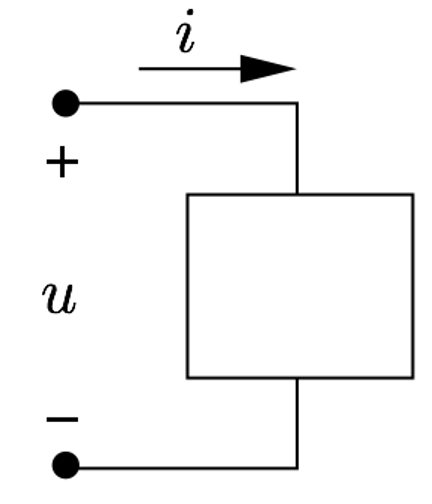
\includegraphics[width=0.5\textwidth]{images/sens_moteur.png} \\
    puissance délivrée \alert{au} dipôle
  \end{column}
  \begin{column}{0.45\textwidth}
    \centering
    Sens non-conventionnel ou \alert{générateur}
    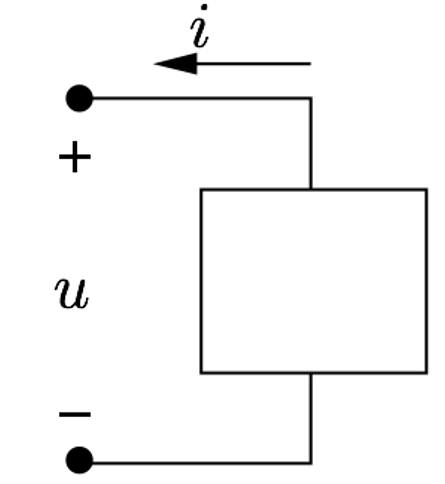
\includegraphics[width=0.5\textwidth]{images/sens_generateur.png} \\
    puissance délivrée \alert{par le} dipôle
  \end{column}
\end{columns}
\end{frame}

\begin{frame} [allowframebreaks] {Exemple}
\begin{columns}
  \begin{column}{0.25\textwidth}
    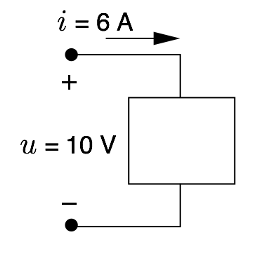
\includegraphics[width=\textwidth]{images/exemple_convention_1.png}
  \end{column}
  \begin{column}{0.7\textwidth}
  Sens \alert{conventionnel} :
    \begin{itemize}
      \item $p=u . i=$ puissance \textbf{délivrée au dipôle}
      \item Signe de $u >0$, potentiel le plus haut à la borne $+$
      \item Signe de $i >0$, charges $+$ entrent par la borne $+$
    \end{itemize}
    $$ p=10.6=60 W $$
    $p=u . i>0$, le dipôle absorbe de la puissance
    Puissance délivrée au dipôle par le reste du circuit = puissance absorbée par le dîpôle
  \end{column}
\end{columns}

\newpage

\begin{columns}
  \begin{column}{0.25\textwidth}
    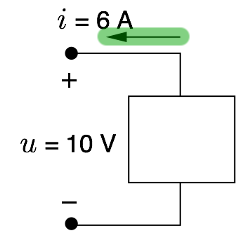
\includegraphics[width=\textwidth]{images/exemple_convention_2.png}
  \end{column}
  \begin{column}{0.7\textwidth}
  Sens \alert{non-conventionnel} :
    \begin{itemize}
      \item $p=u . i=$ puissance \textbf{fournie par le} dipôle
      \item Signe de $u >0$, potentiel le plus haut à la borne $+$
      \item Signe de $i >0$, charges $+$ entrent par la borne $-$
    \end{itemize}
    $$ p=10.6=60 W $$
    $p=u . i>0$, le dipôle fournit de la puissance.\\
    Puissance \textbf{délivrée au} dipôle: $-u.i=-60 W$.
  \end{column}
\end{columns}
  \newpage

\begin{columns}
  \begin{column}{0.25\textwidth}
    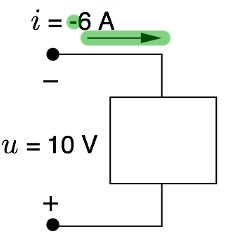
\includegraphics[width=\textwidth]{images/exemple_convention_3.png}
  \end{column}
  \begin{column}{0.7\textwidth}
  Sens \alert{non-conventionnel} :
    \begin{itemize}
      \item $p=u . i=$ puissance \textbf{fournie par le} dipôle
      \item Signe de $u >0$, potentiel le plus haut à la borne $+$
      \item Signe de $i <0$, charges $+$ entrent par la borne $+$
    \end{itemize}
    $$ p=10.(-6)=-60 W $$
    $p=u . i<0$, le dipôle absorbe de la puissance.\\
    Puissance \textbf{absorbée par le} dipôle: $-u.i=60 W$.
  \end{column}
\end{columns}
\end{frame} 

\begin{frame}{Elements actifs et passifs}
Soit $p(t) \in \mathbb{R} $ la puissance fournie à un dipôle.
L'énergie fournie au dipôle est
$$
w(t)=\int_{-\infty}^t p(\tau) d \tau
$$

\begin{tabular}{c|c} 
Elément passif & \multicolumn{1}{|c}{ Elément actif } \\
\hline$w(t) \geq 0 \quad \forall t$ & $\exists t: w(t)<0$ \\
\begin{tabular}{c} 
ne restitue jamais plus d'énergie \\
qu'il n'en a reçu \\
exemple : résistance
\end{tabular} & \begin{tabular}{l} 
peut fournir une certaine quantité \\
d'énergie \\
exemple : source de tension (pile)
\end{tabular}
\end{tabular}  
%  \begin{itemize}
%    \item 
%    \item 
%  \end{itemize}
%
%\begin{columns}
%  \begin{column}{0.45\textwidth}
%    
%    % \centering
%    % 
\includegraphics[width=0.3\textwidth]{images/run.png}
%  \end{column}
%  \begin{column}{0.45\textwidth}
%    
%  \end{column}
%\end{columns}
\end{frame}

\begin{frame}{Nous avons établi la formule permettant de déterminer la résistance équivalente à la mise }
  
\begin{columns}
  \begin{column}{0.45\textwidth}
    \alert{en série} de plusieurs résistances : $$\boxed{R_{eq} = \sum_{i=1}^n R_i}$$
    \centering
    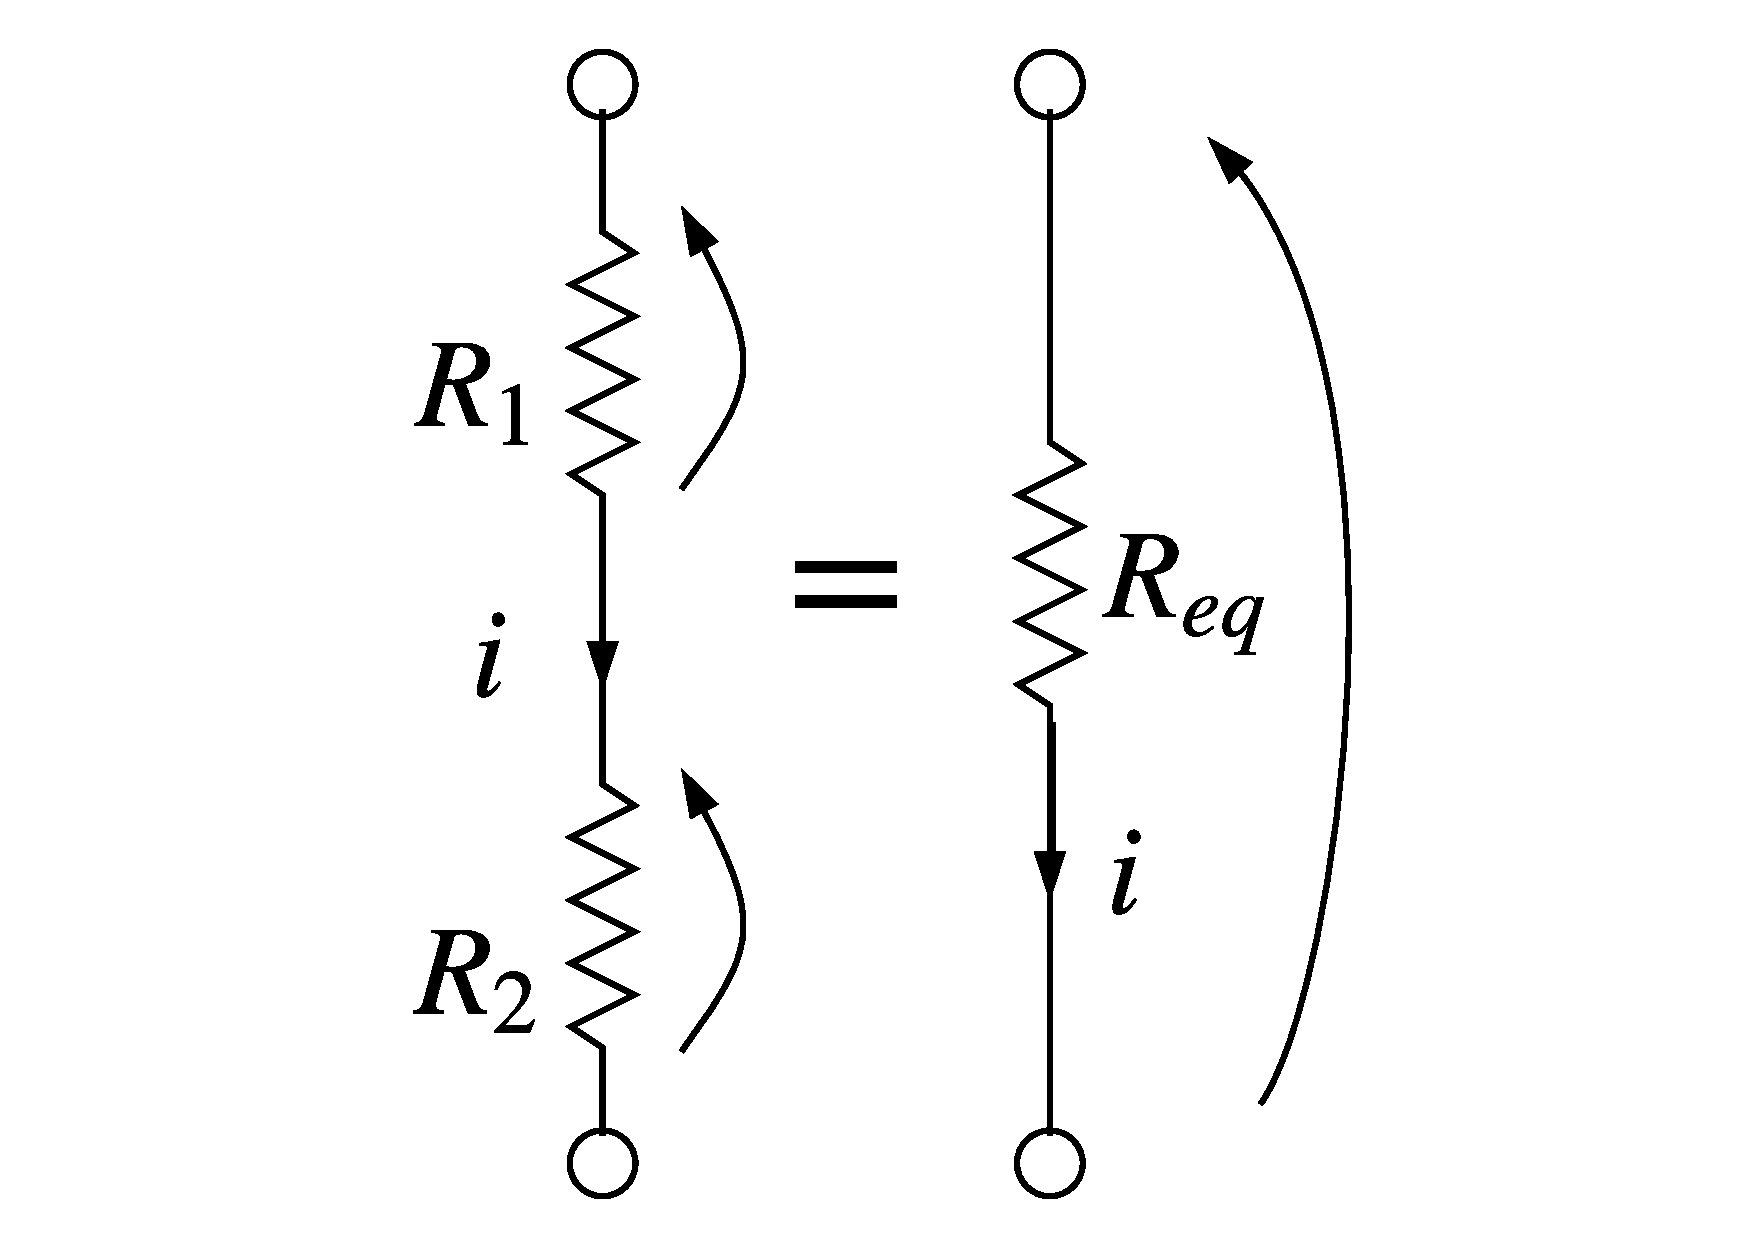
\includegraphics[width=0.6\textwidth]{images/serie.pdf}
  \end{column}
  \begin{column}{0.45\textwidth}
    \alert{en parallèle} de plusieurs résistances : $$\boxed{R_{eq} = \left(\sum_{i=1}^n \frac{1}{R_i}\right)^{-1}}$$
    \centering
    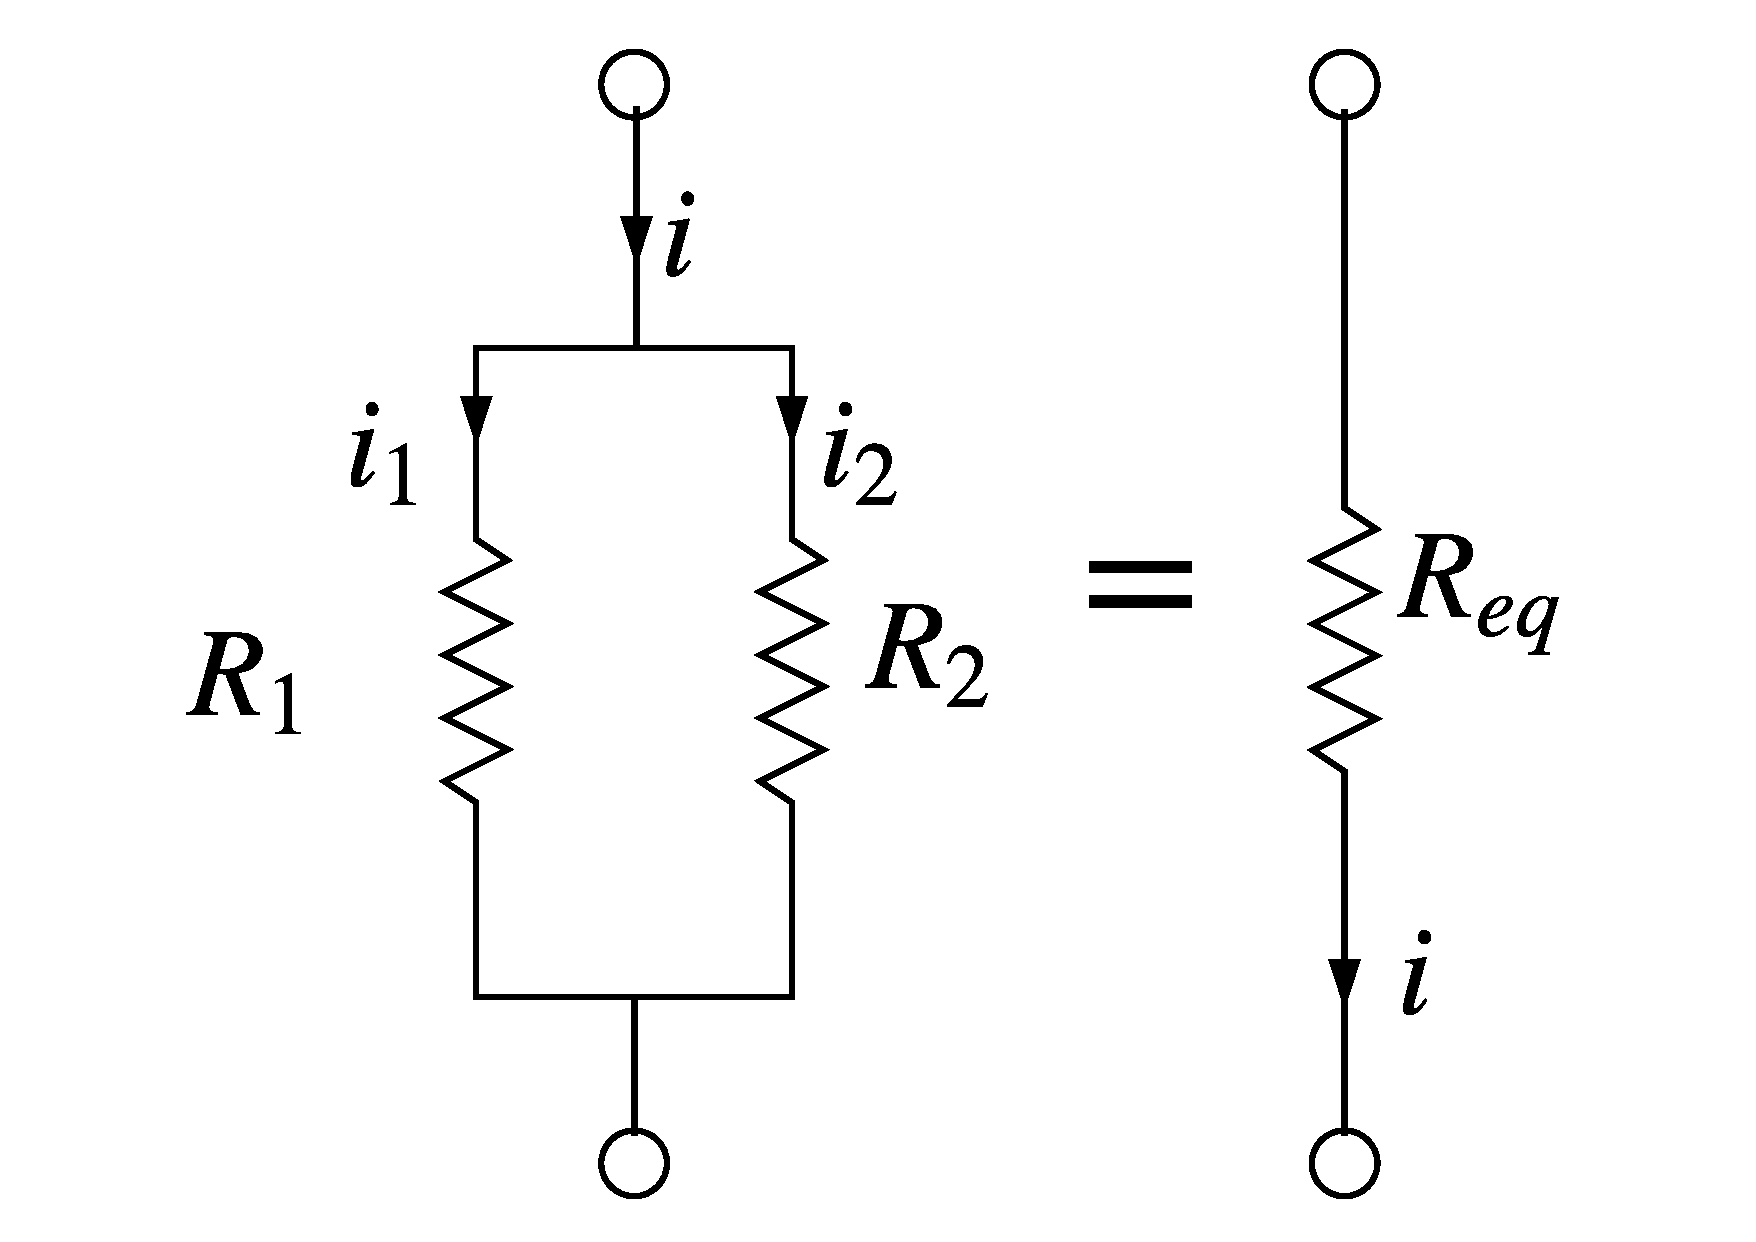
\includegraphics[width=0.6\textwidth]{images/parallele.pdf}
  \end{column}
\end{columns}
\end{frame}

\begin{frame}{Diviseurs de tension et de courant}
  
\begin{columns}
  \begin{column}{0.45\textwidth}
      Formule du \alert{diviseur de tension}.
	
		$$ \boxed{U = E \frac{R_L}{R_L+R_i}}$$
	
    \centering
    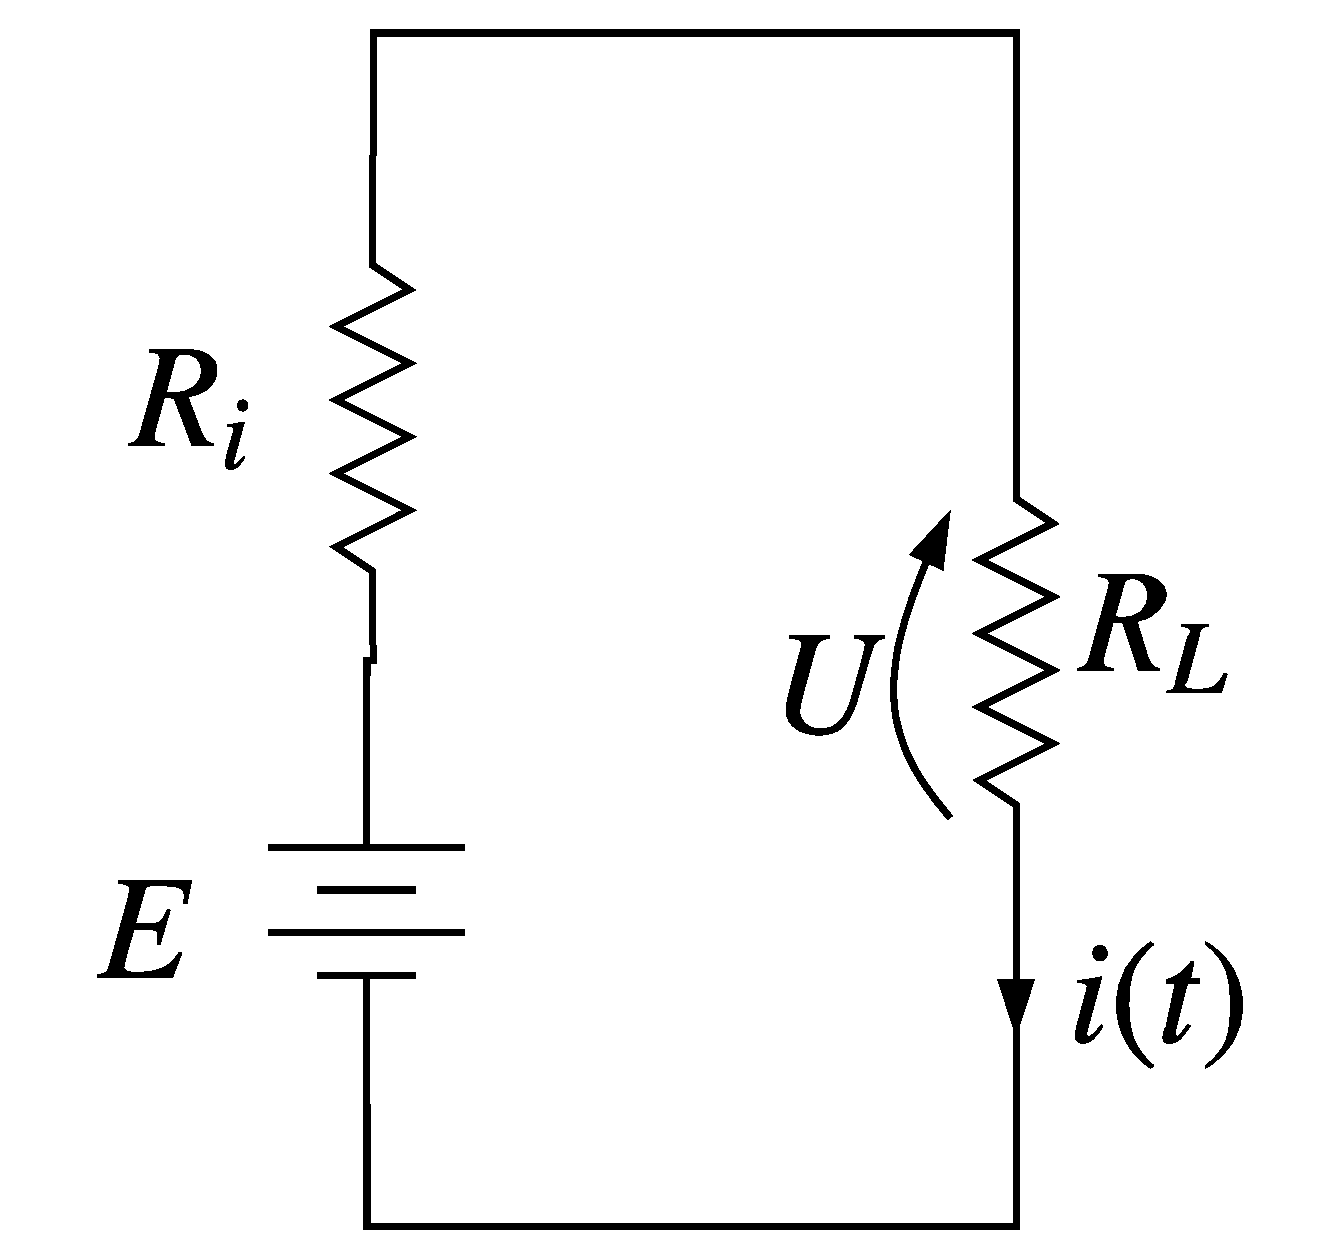
\includegraphics[width=0.5\textwidth]{images/SourceReelleV.pdf}
  \end{column}
  \begin{column}{0.45\textwidth}
      Formule du \alert{diviseur de courant}.
	
		$$ \boxed{I = J \frac{G_L}{G_L+G_i}}$$

    \centering
    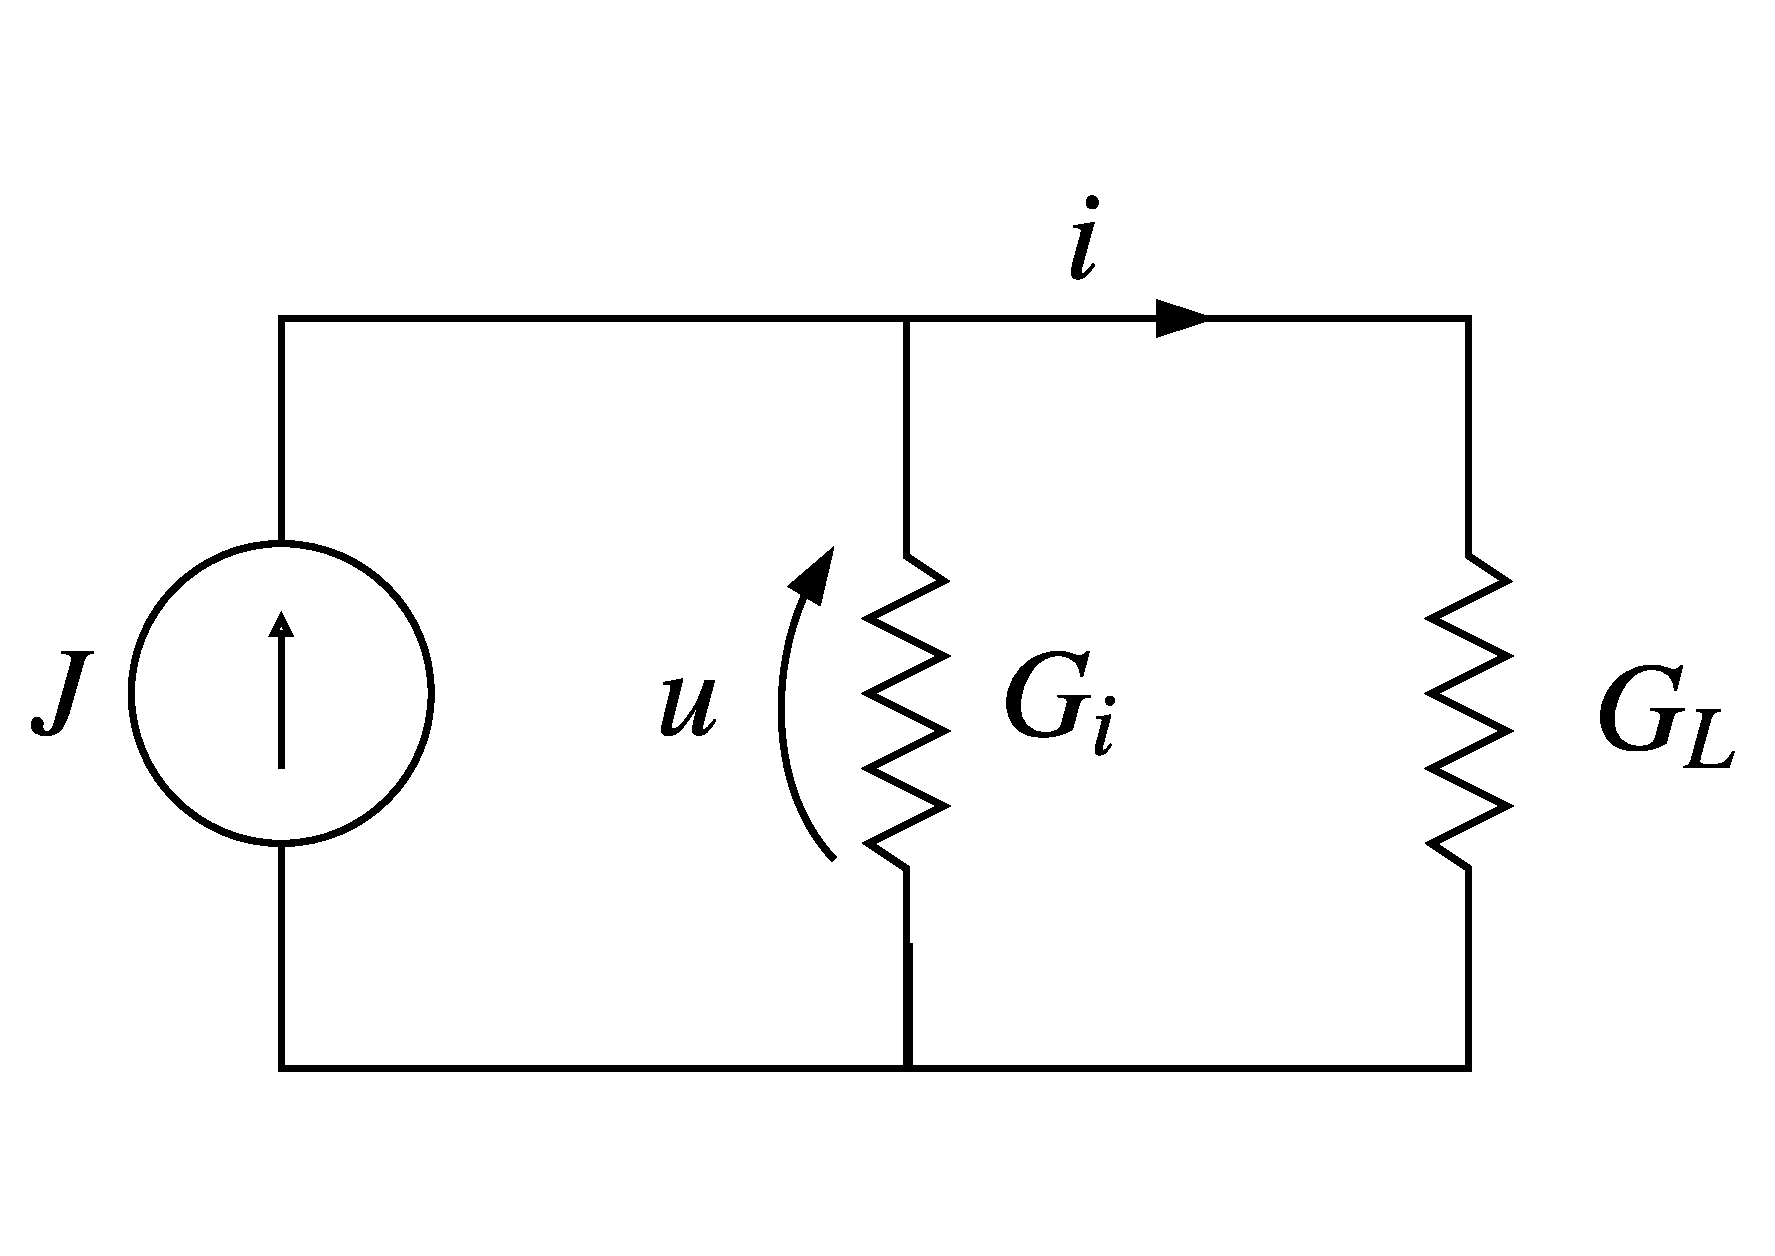
\includegraphics[width=0.7\textwidth]{images/SourceDeCourantReelle.pdf}

  \end{column}
\end{columns}

Ces deux figures illustrent la notion de source indépendante de tension (gauche) et de courant (droite) et leur modèle "réaliste" avec l'ajout de $R_i$ et de $G_i$, respectivement.
\end{frame}

\begin{frame}{Qu'allons nous faire dans ce cours ?}
  
  \begin{itemize}
    \item Nous étudions de nouveaux éléments: les condensateurs (C) et les bobines (L). 
    \item Ces éléments introduisent une dynamique dans les circuits lorsqu'il y a des commutations ou des excitations qui varient avec le temps. 
    \item Nous apprenons comment caractériser cette dynamique. 
    \item Notions mathématiques utilisées 
    \begin{itemize}
      \item les équations différentielles du premier et du second ordre, à coefficients constants. 
      \item les nombres complexes, exponentielle de nombre complexes, fonctions hyperboliques. 
    \end{itemize}
  \end{itemize}
\end{frame}


\section{Sources commandées}

\begin{frame}{Définition}
  \begin{columns}
  \begin{column}{0.4\textwidth}
    Une source commandée est un quadripôle unidirectionnel, non-autonome et actif ; un de ses accès est celui qui exerce la commande (accès de commande), l'autre est l'accès commandé.
    
    Autrement dit, la tension ou le courant délivré par la source dépend de la valeur d'une d.d.p ou d'un courant à un autre endroit du circuit.  
  \end{column}
  \begin{column}{0.5\textwidth}

    \begin{center}
      Exemple : source VVT (\textit{}voltage to voltage transducer)
      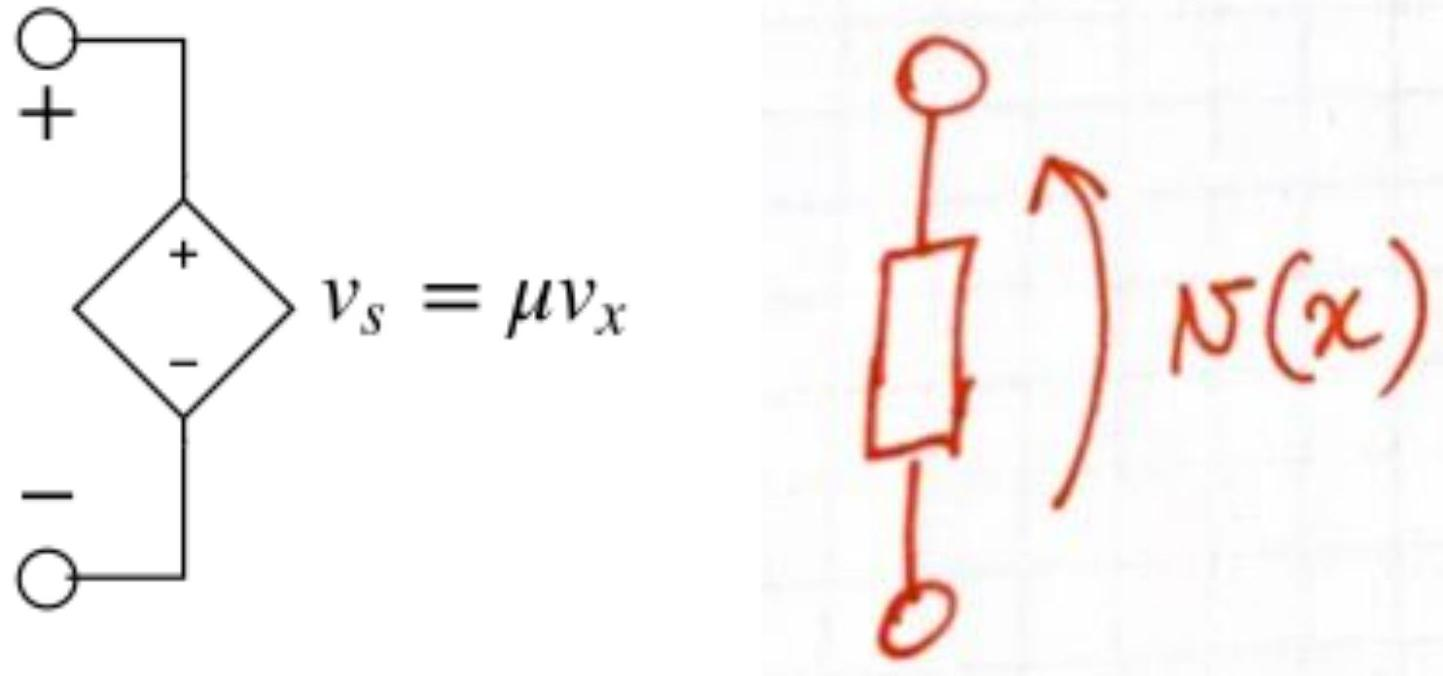
\includegraphics[width=0.8\textwidth]{images/0aae1f8e-05fc-4834-a308-b46d85861175-17_676_1443_660_2796}
    \end{center}
    \begin{itemize}
      \item $v_{s}$ n'est déterminé à l'instant $t$ que si la valeur $v_{x}(t)$ est connue
      \item $v_{x}$ est la tension de commande et $v_{s}$ la tension commandée
    \end{itemize}
  \end{column}
\end{columns}


\end{frame}

\begin{frame}{Propriétés}
Puisque les relations de dépendance introduites ci-dessus sont linéaires, ces sources commandées sont des éléments linéaires.

Les sources dépendantes ne sont pas des excitations :

\begin{itemize}
  \item analogues à des éléments résistifs, elle introduisent un couplage entre différentes branches du circuit.
\end{itemize}

Comme nous le verrons au Chapitre 7, les sources commandées sont utiles pour la modélisation de circuits électroniques.

\end{frame}

\begin{frame}{Il en existe de quatre types}

  \begin{columns}
  \begin{column}{0.45\textwidth}
    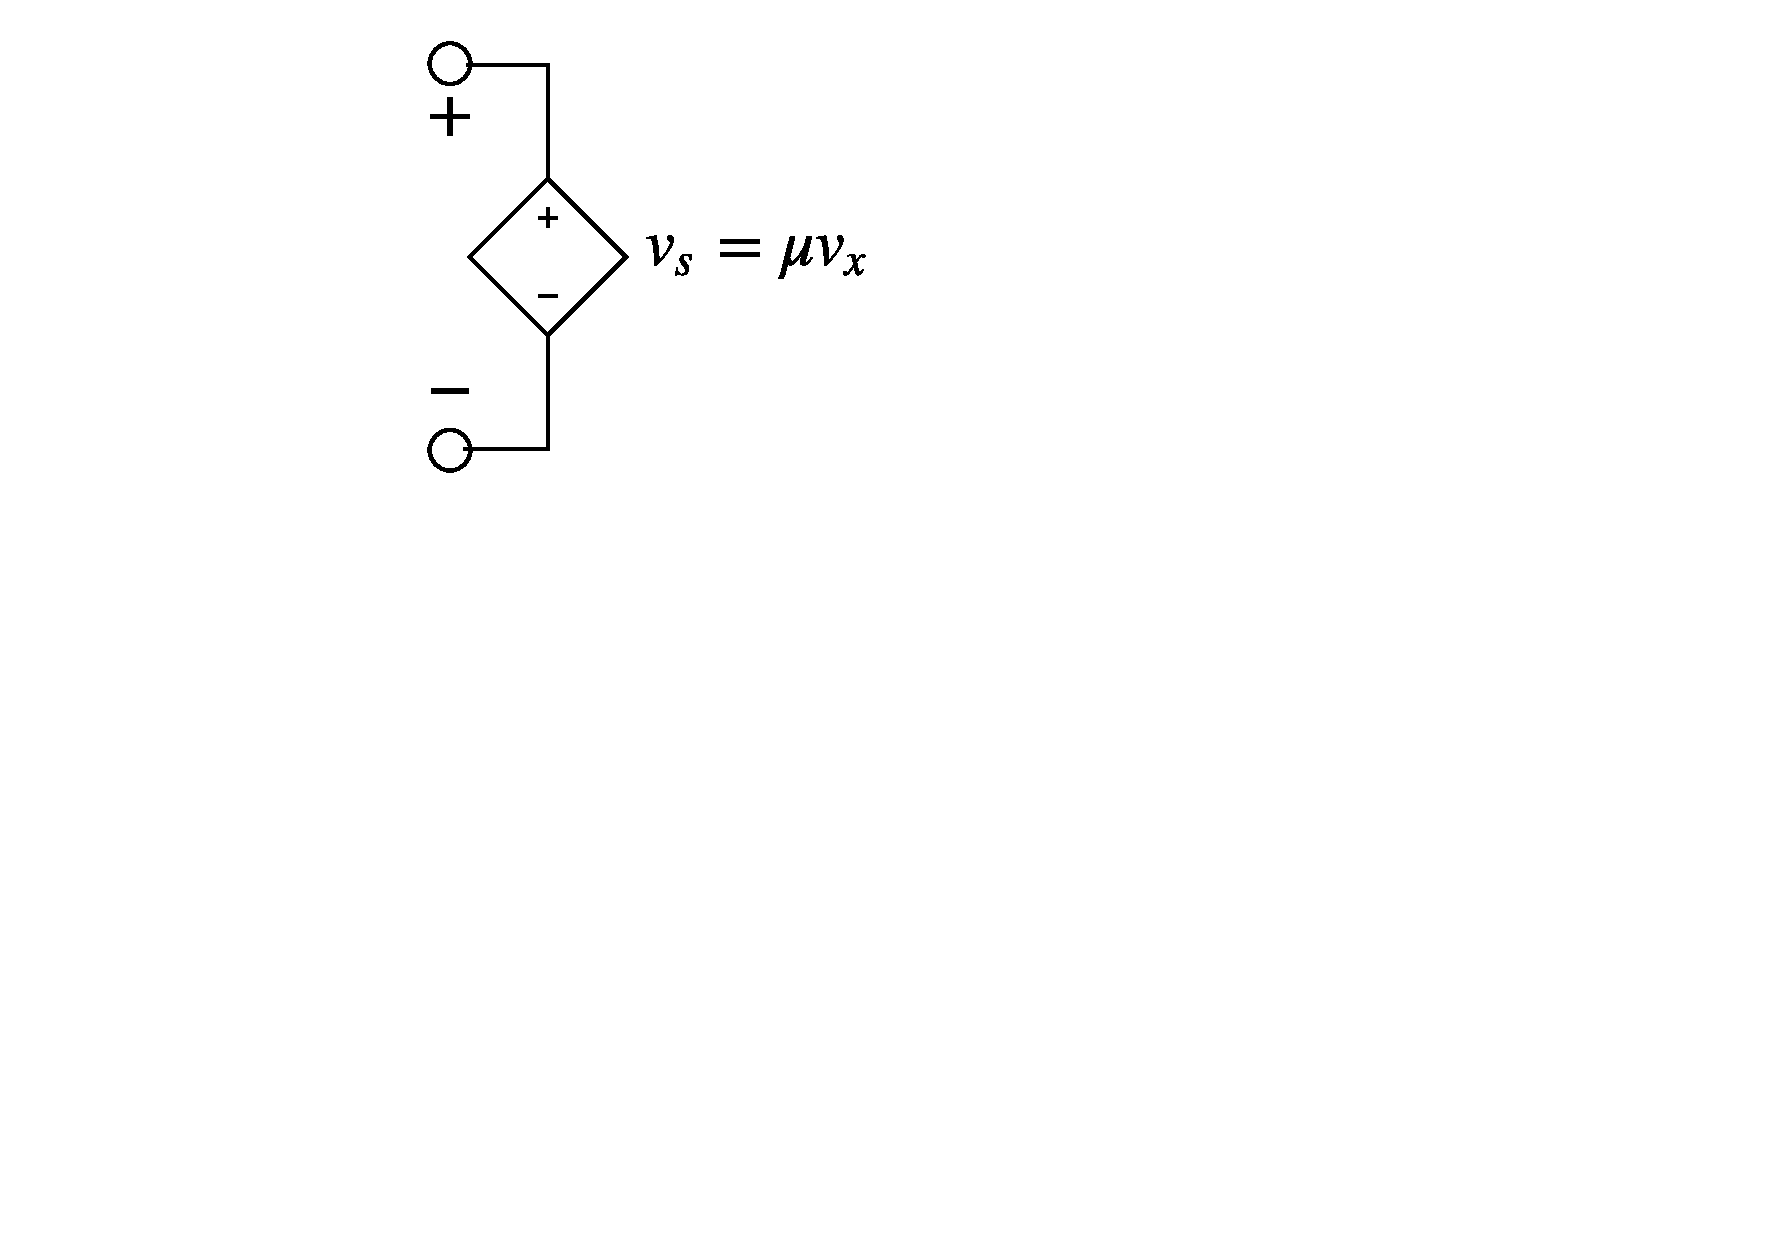
\includegraphics[width=0.5\textwidth]{images/VVT.pdf}
    \textbf{VVT} 

  \end{column}
  \begin{column}{0.45\textwidth}
    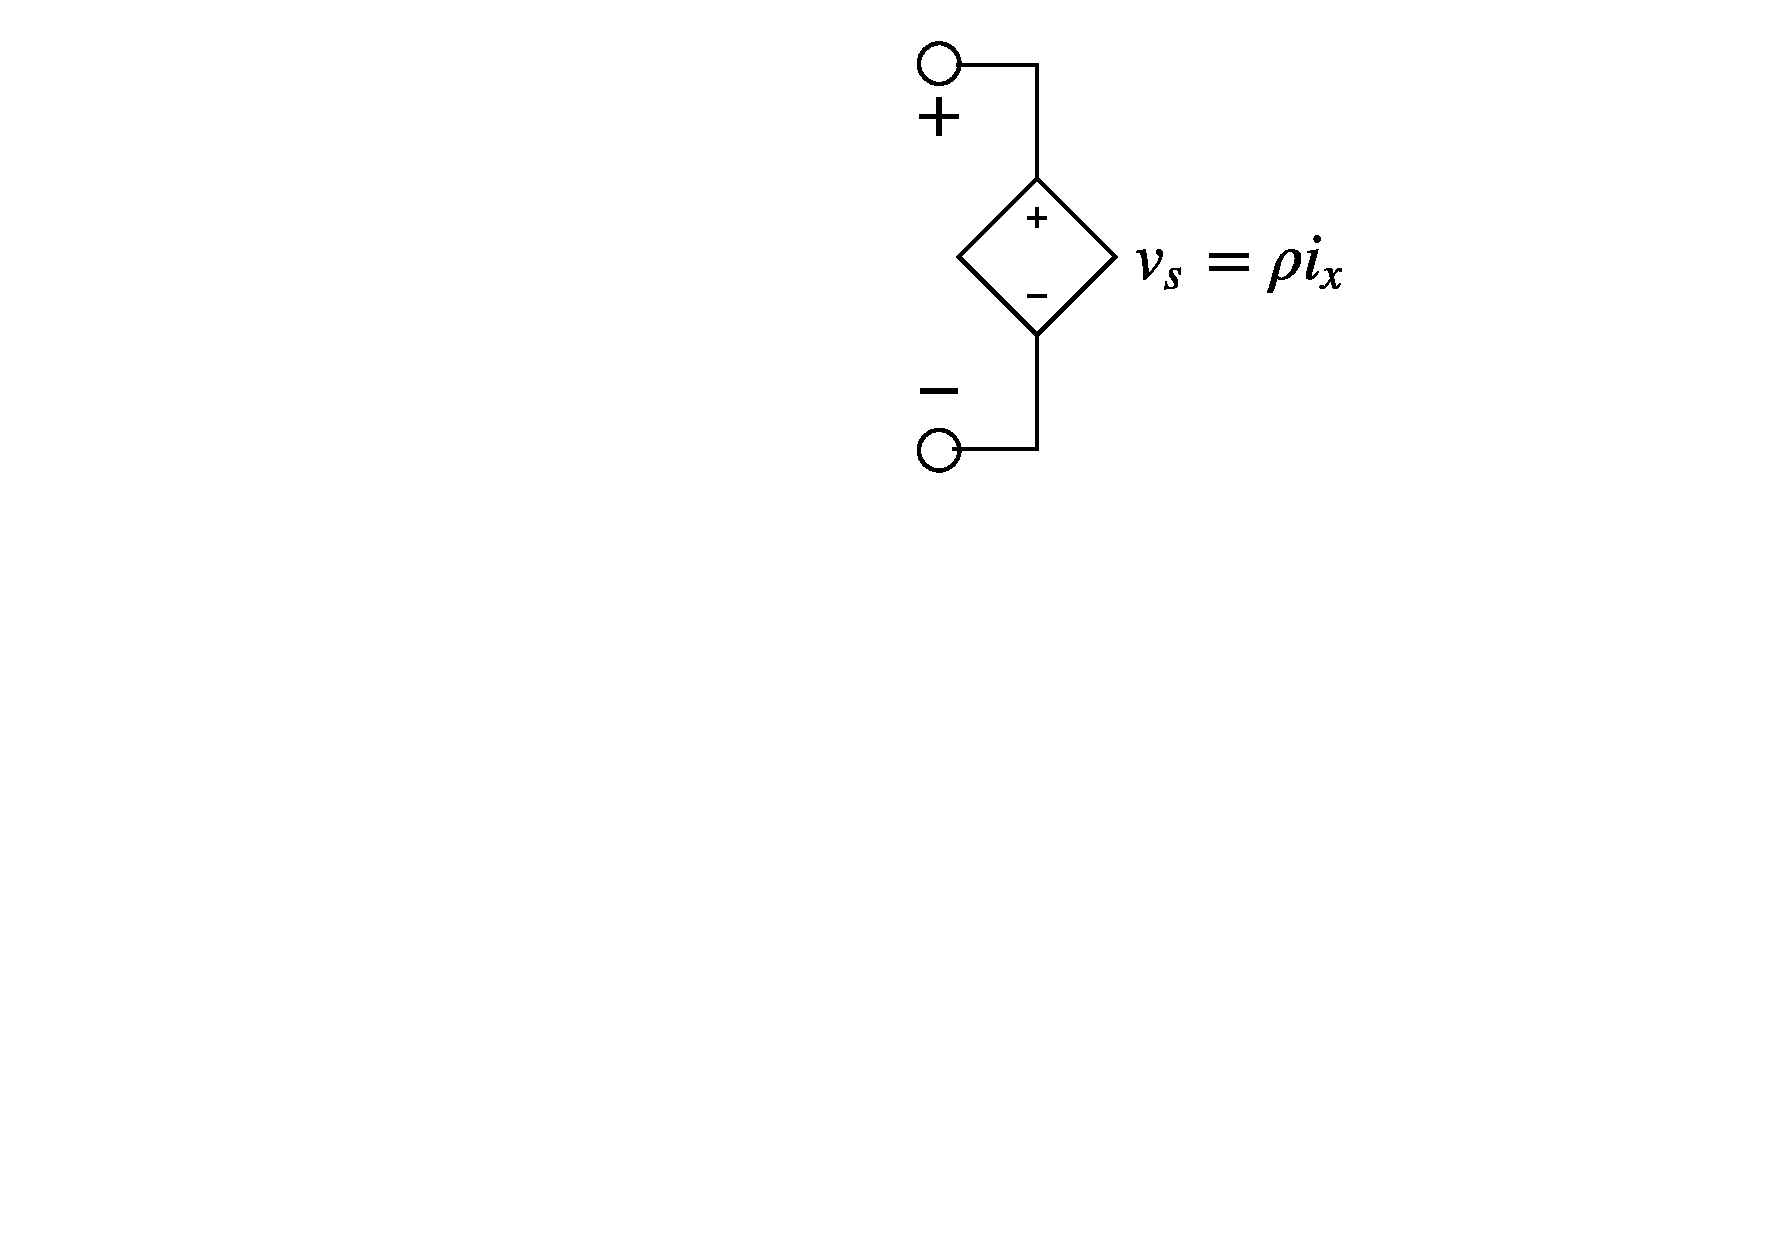
\includegraphics[width=0.5\textwidth]{images/CVT.pdf}
    \textbf{CVT},     $\rho[\Omega]$

  \end{column}
  \end{columns}

  \begin{columns}
  \begin{column}{0.45\textwidth}
    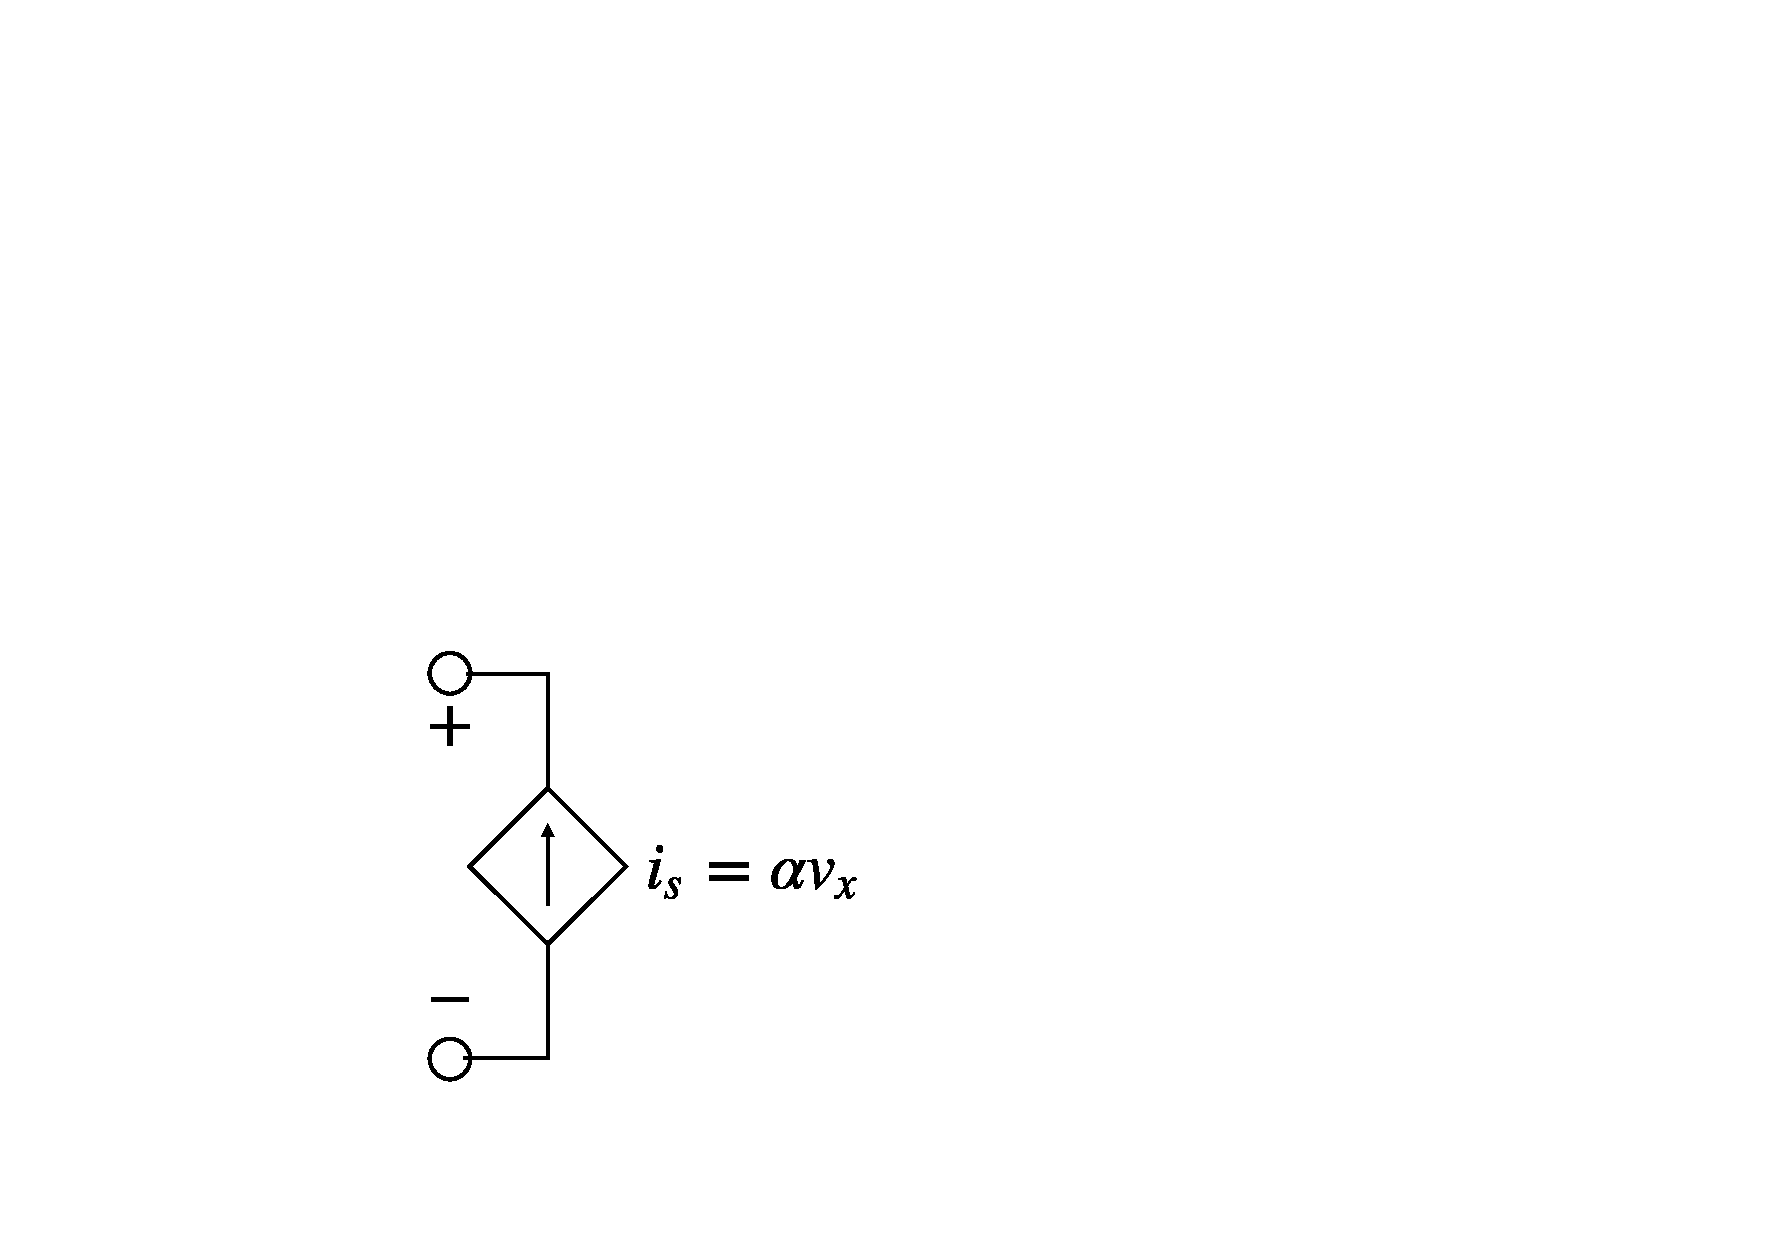
\includegraphics[width=0.5\textwidth]{images/VCT.pdf}
    \textbf{VCT}, $\alpha [S]$ 

  \end{column}
  \begin{column}{0.45\textwidth}
    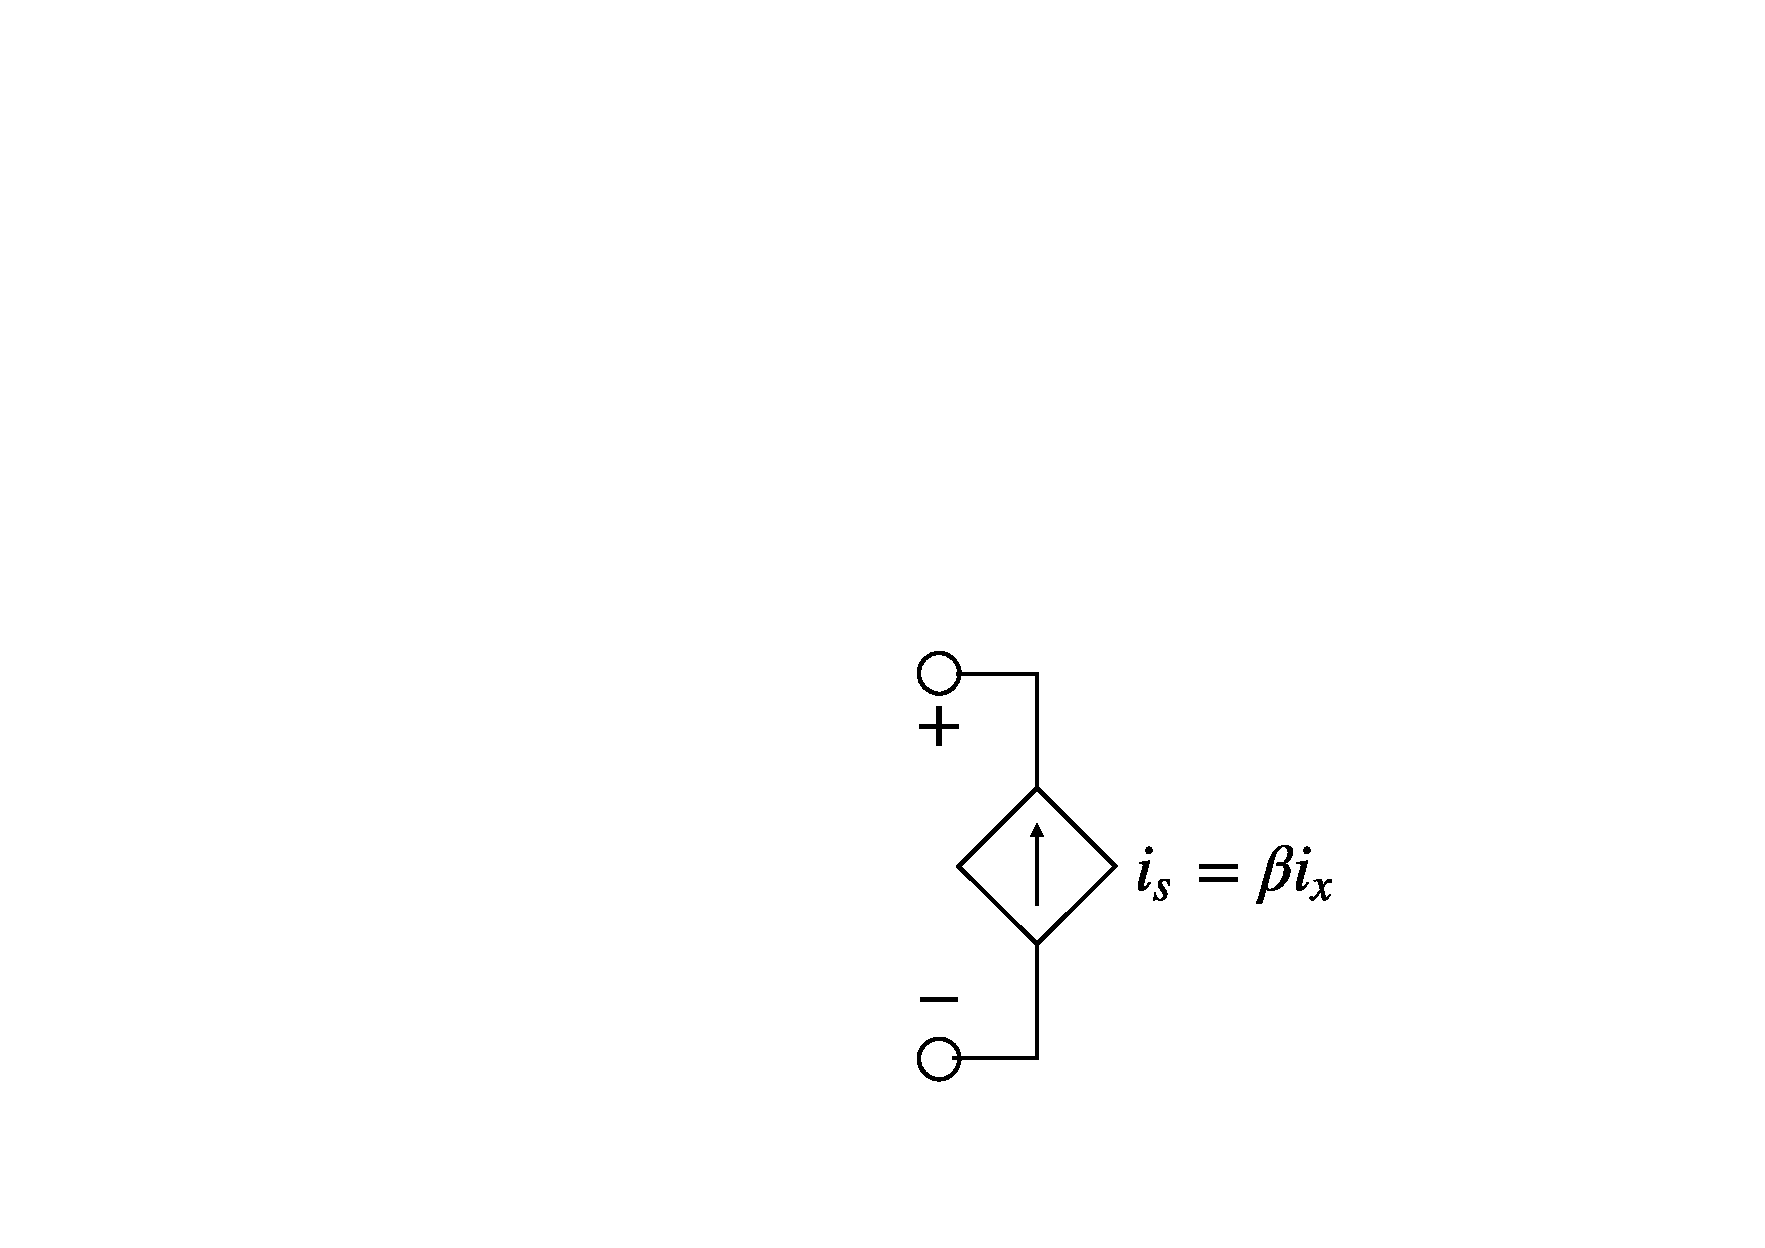
\includegraphics[width=0.5\textwidth]{images/CCT.pdf}
    \textbf{CCT}  
  \end{column}
  \end{columns}  
\end{frame}

\section{Condensateurs} 

\begin{frame}{Condensateur plan en régime stationnaire}
  

\begin{columns}
  \begin{column}{0.3\textwidth}
    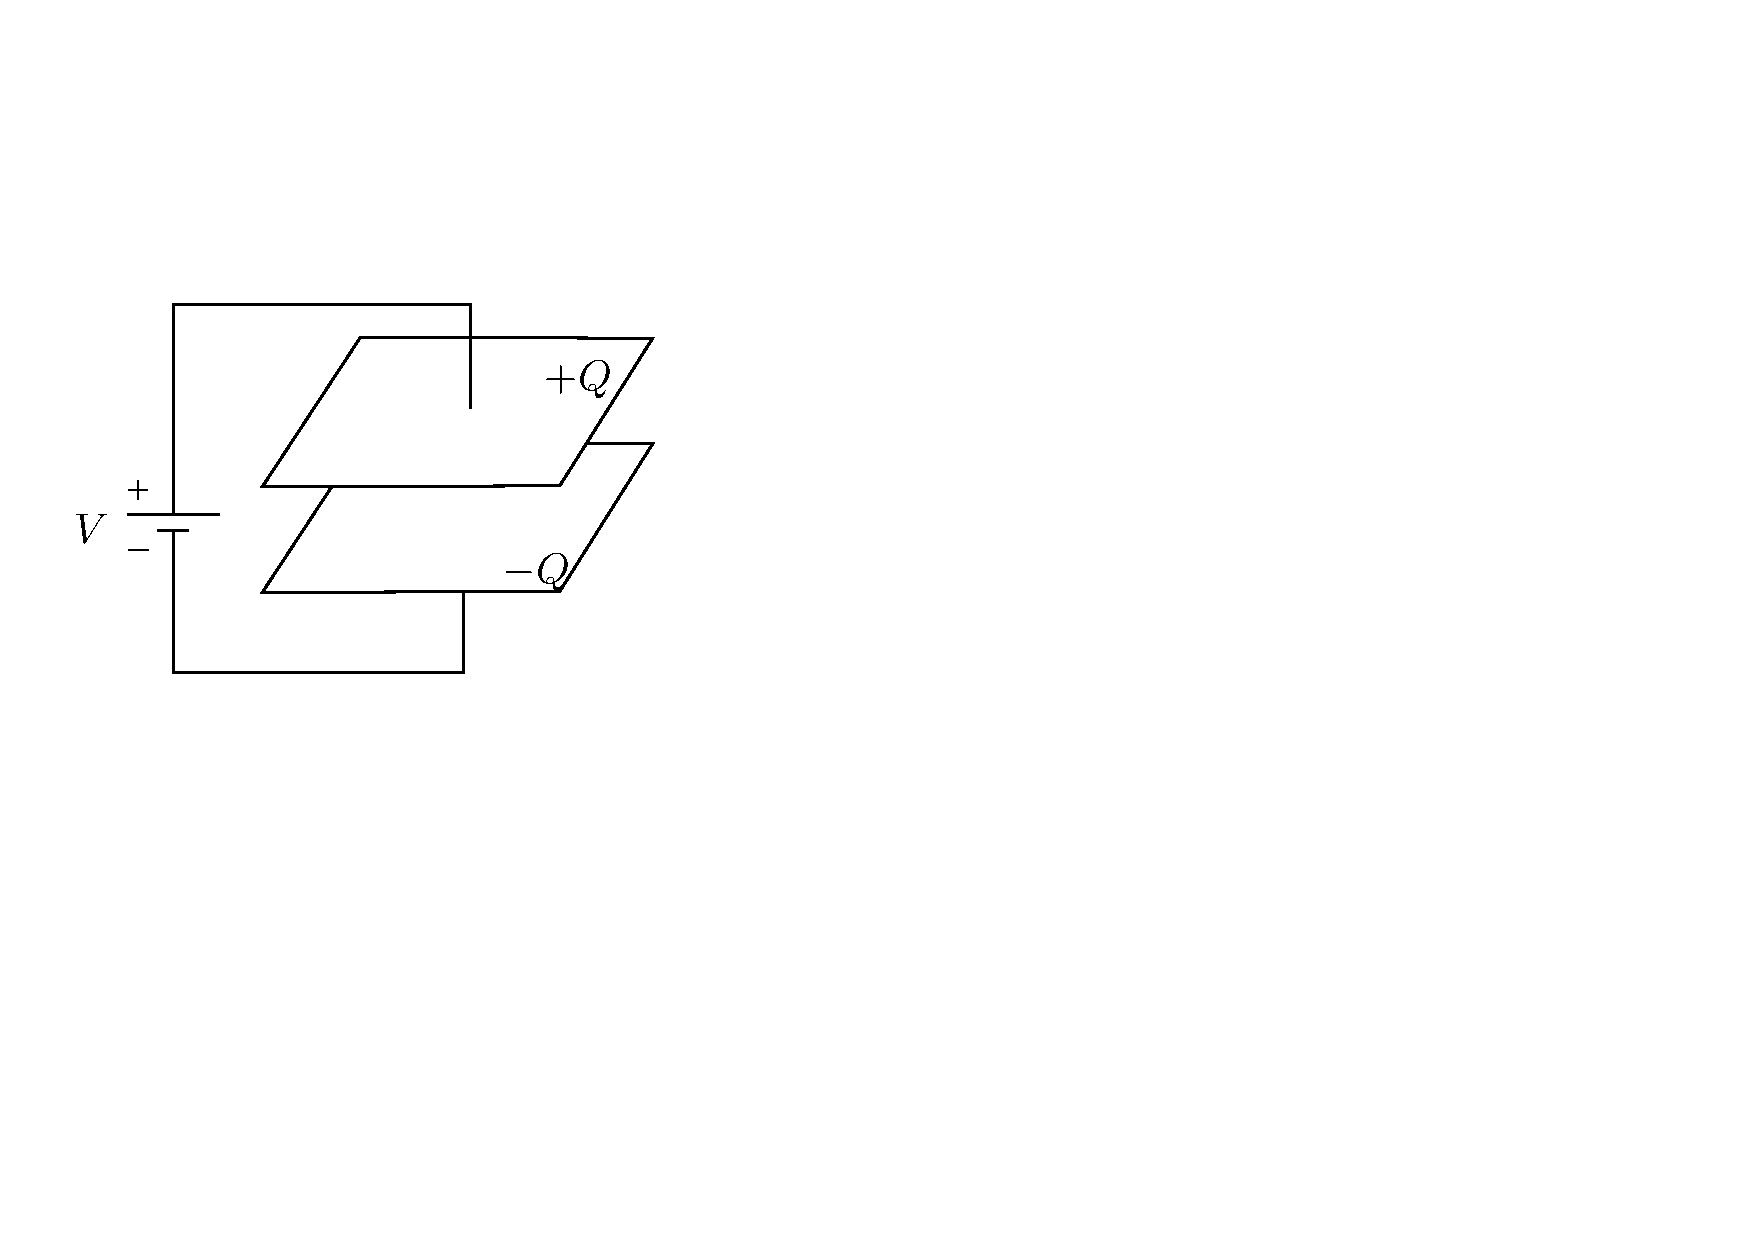
\includegraphics[width=4cm]{images/condensateur.pdf}  
  \end{column}
  \begin{column}{0.65\textwidth}

    Un condensateur est constitué de deux plaques parallèles conductrices de surface $S$ séparées d'une distance $d$ et portant des charges égales et opposées $\pm Q$. \\[3mm]

    Les charges font naître une différence de potentiel $V$ entre les plaques.
  \end{column}
\end{columns}
\vspace{5mm}

$C$, le coefficient de proportionnalité entre $Q$ et $V$, est appelé \alert{capacité du condensateur}: 
$$\boxed{C = \frac{Q}{V}}$$
\end{frame}

\begin{frame} {Paramètres physiques d'un condensateur et capacité}
La capacité s'exprime, en fonction des paramètres physiques du condensateur par 
$$\boxed{C=\frac{\epsilon S}{d}}$$ où $\epsilon$ est la \textbf{permittivité diélectrique} du matériau placé entre les plaques.

La capacité s'exprime en \alert{farad}, dont le symbole est $F$.

\textbf{En toute généralité}, $C$ est fonction de la tension à ses bornes, du courant et peut varier avec le temps.
\end{frame}

\begin{frame} {En régime non stationnaire}
Une variation du potentiel $V$ implique une modification de la charge
portée par les plaques conductrices. Cette variation est apportée par
un circuit extérieur débitant un courant.

Au niveau du condensateur :
\begin{itemize}
	\item la différence de  potentiel à ses bornes varie
	\item le champ électrique $\overrightarrow{E}$ dans le matériau
	diélectrique placé entre les plaques est variable
	\item il existe un {\em courant de déplacement}.
	\[\vec{\nabla} \times \overrightarrow{H}  = 
	\frac{\partial \overrightarrow{D}}{\partial t}\]
\end{itemize}
Ce courant de déplacement et ce champ électrique variable sont
``confinés'' à l'intérieur de l'élément, car on fait l'hypothèse des circuits
localisés.
\end{frame}

\begin{frame}[allowframebreaks] {Relation tension-courant}

\textbf{En pratique}, dans ce cours,  nous allons toujours considérer la capacité $C$ linéaire et invariante $\Rightarrow$ constante.
\vspace{\baselineskip}
\begin{columns}
  \begin{column}{0.45\textwidth}
  On appelle condensateur un dipôle tel que la charge $q$ induite par une d.d.p. $u$ à ses bornes est une fonction de cette d.d.p.
  $$
  q(t)=C u(t)
  $$
  Comme le courant $i(t)$ est défini par 
  $$i(t)=\frac{dq(t)}{dt}$$  
  \end{column}
  \begin{column}{0.45\textwidth}
  on a aux bornes d'un condensateur
  $$\boxed{i(t)=C\frac{du(t)}{dt}}$$
  ou encore 
  $$ \quad u(t) = \frac{1}{C}\int_{-\infty}^t i(\tau) d\tau.$$
  \end{column}
\end{columns}


\begin{columns}
  \begin{column}{0.45\textwidth}
    Ces relations sont établies selon le \textbf{sens conventionnel} !
  \end{column}
  \begin{column}{0.45\textwidth}
    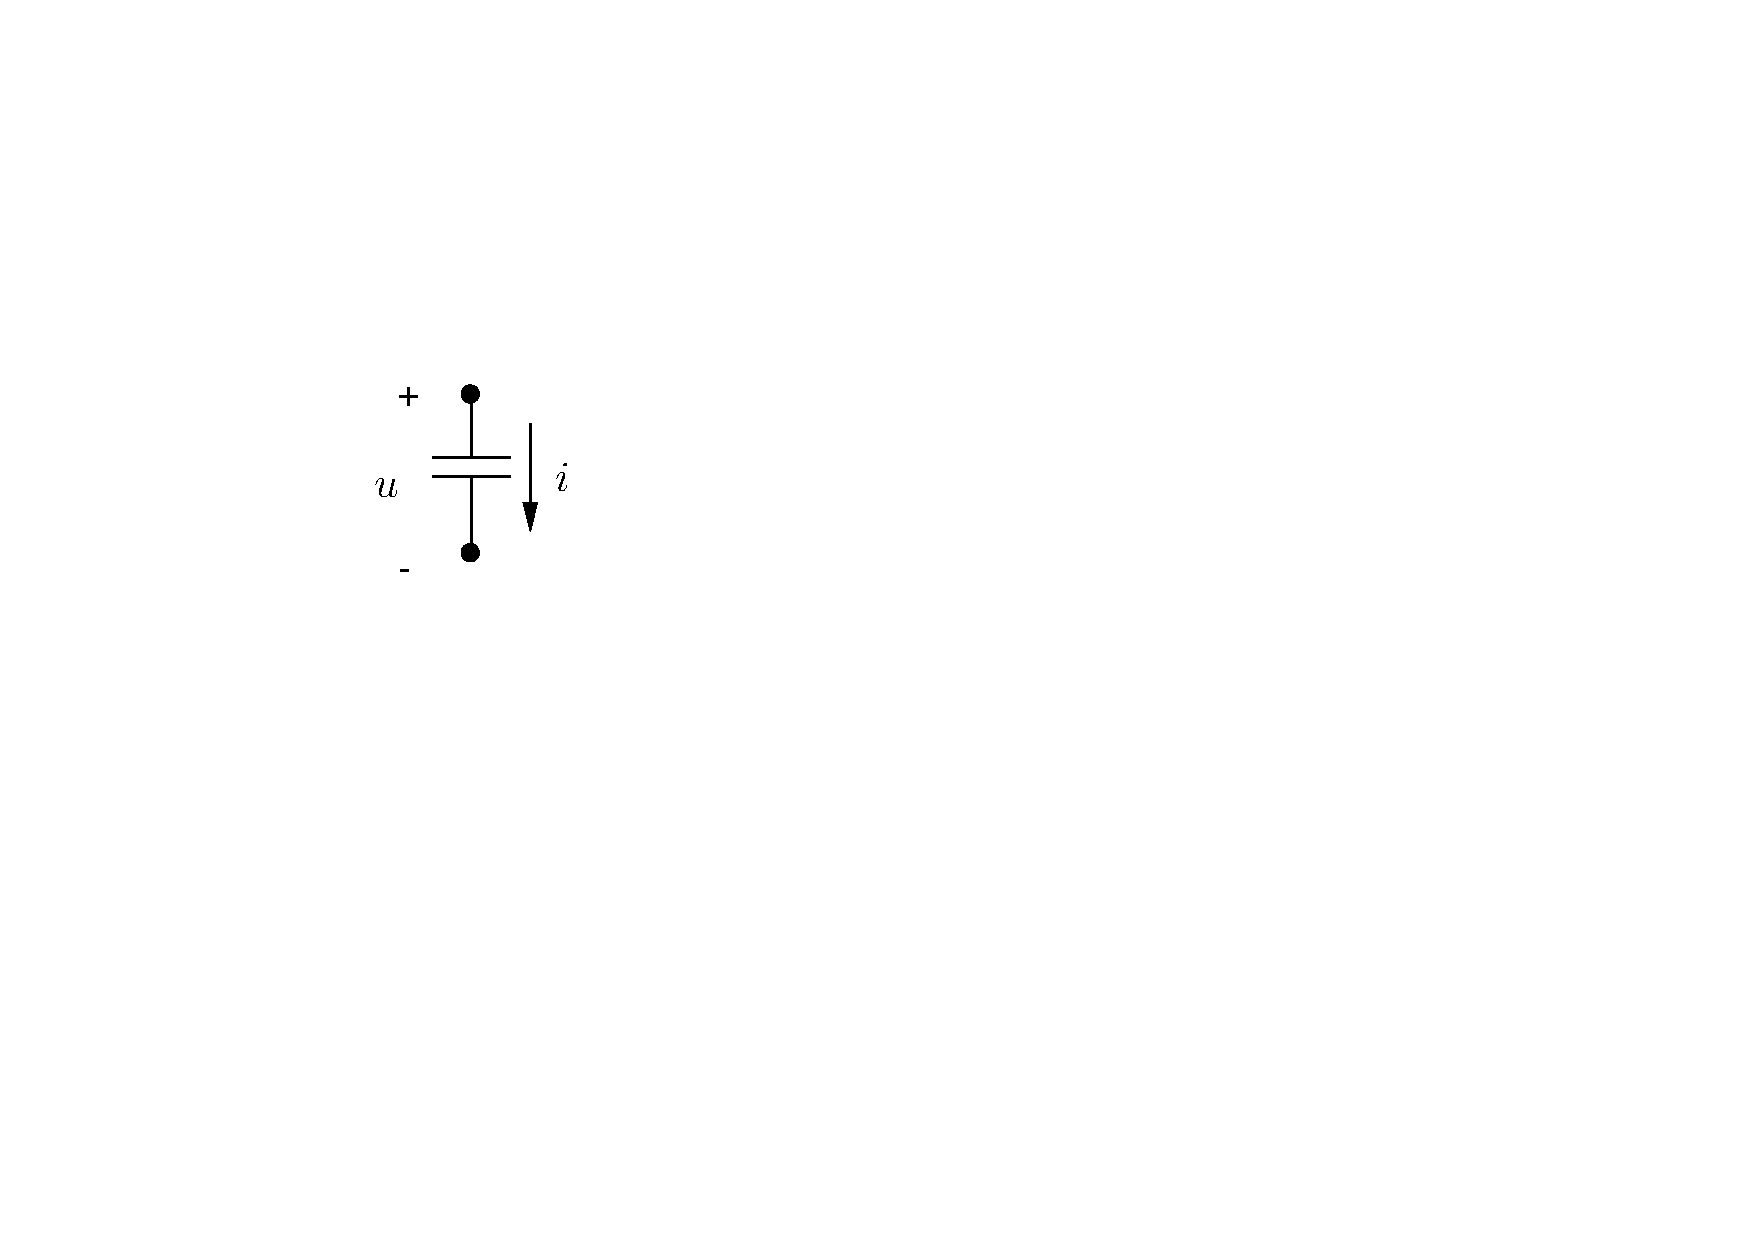
\includegraphics[width=4cm]{images/symbole_condensateur_et_sens.pdf}
  \end{column}
\end{columns}

\end{frame}



\begin{frame} {En pratique}

\begin{columns}
  \begin{column}{0.5\textwidth}
  Il existe beaucoup d'implémentations physiques et chimiques de condensateur à diélectrique à film plastique (polypropylène, polyester, ...), céramique, au mica, électrolytique, à papier paraffiné, variable à lame d'air (une plaque mobile), etc. \\[5mm]

  Habituellement, on indique la capacité d'un condensateur en $pF$, $nF$ ou $\mu F$.
  \end{column}
  \begin{column}{0.4\textwidth}
    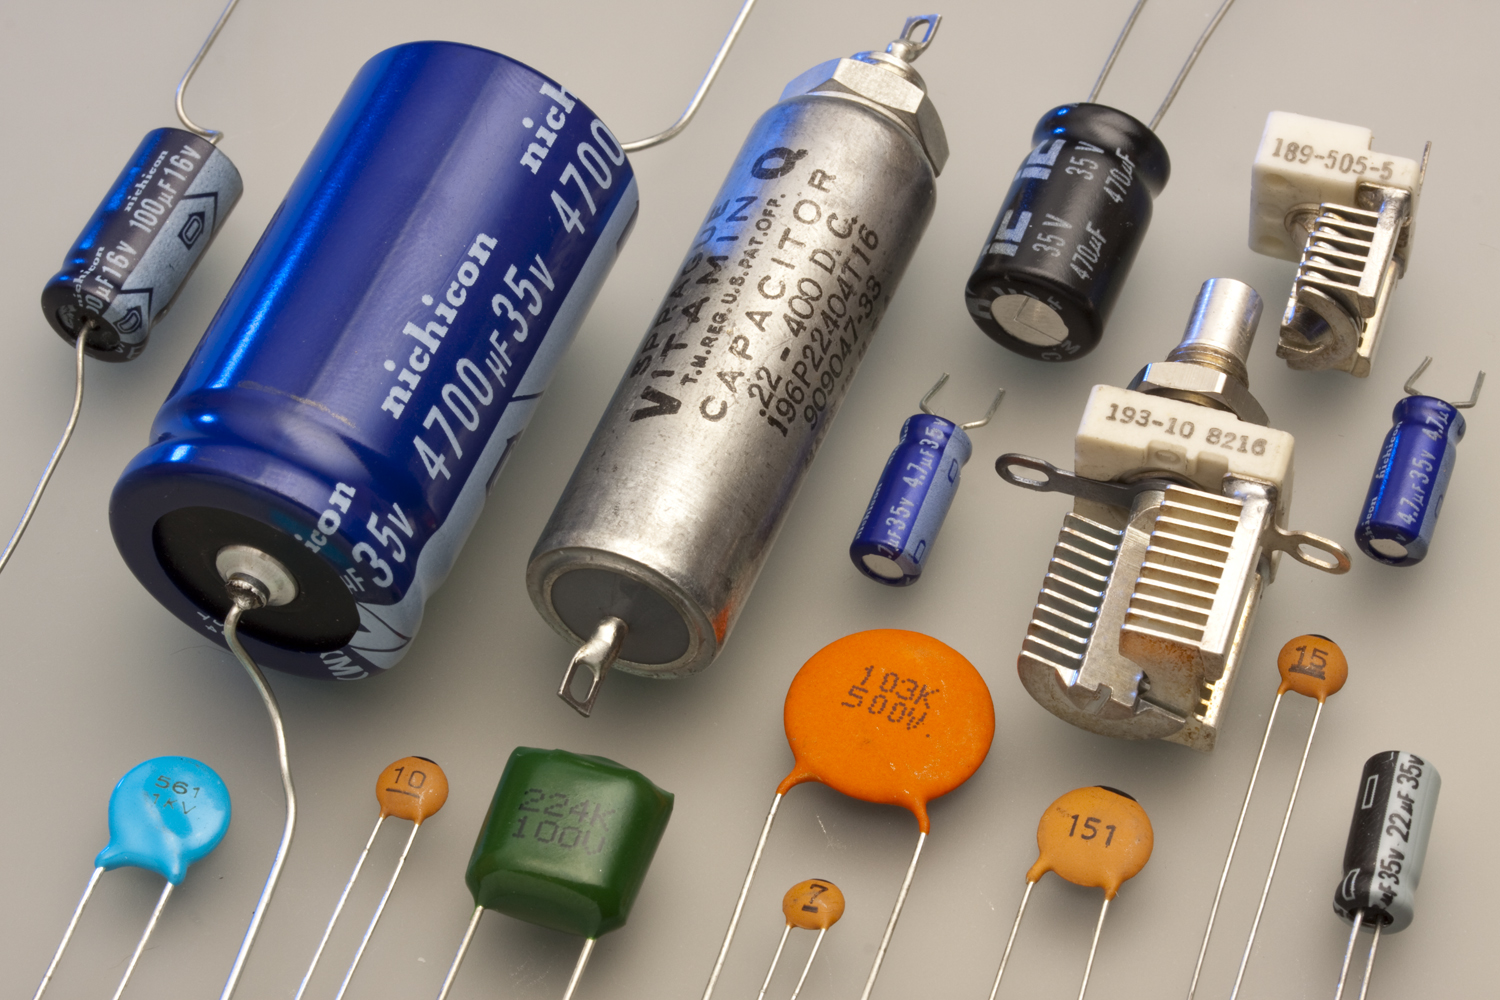
\includegraphics[width=0.9\linewidth]{images/capacitors.jpg} \\
    Exemples des condensateurs. \\ Source: \href{https://fr.wikipedia.org/wiki/Condensateur}{Wikipedia} 
  \end{column}
\end{columns}
\end{frame}


\section{Bobines - inductances}

\begin{frame}{Inductance du solénoïde}
  \begin{columns}
  \begin{column}{0.35\textwidth}
    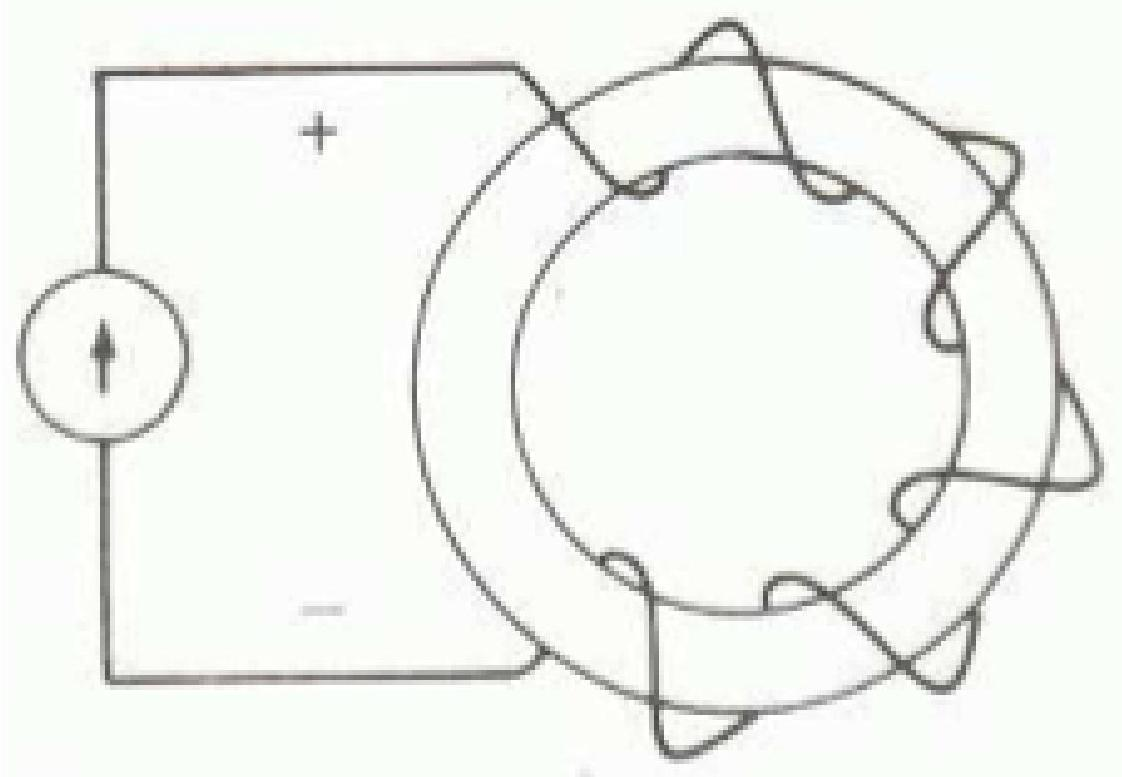
\includegraphics[width=\textwidth]{images/0aae1f8e-05fc-4834-a308-b46d85861175-29_777_1122_662_241}
  \end{column}
  \begin{column}{0.65\textwidth}
    Un noyau magnétique entouré d'une bobine de $N$ spires parcourue par un courant continu $I$ fait naître dans la bobine un flux $\phi$ (flux total embrassé par toutes les spires)
    $$ \phi[W b] $$
  \end{column}
\end{columns}
\begin{center}
\end{center}

Le coefficient de self-induction de cette bobine est $L=\frac{\phi}{I}$.

%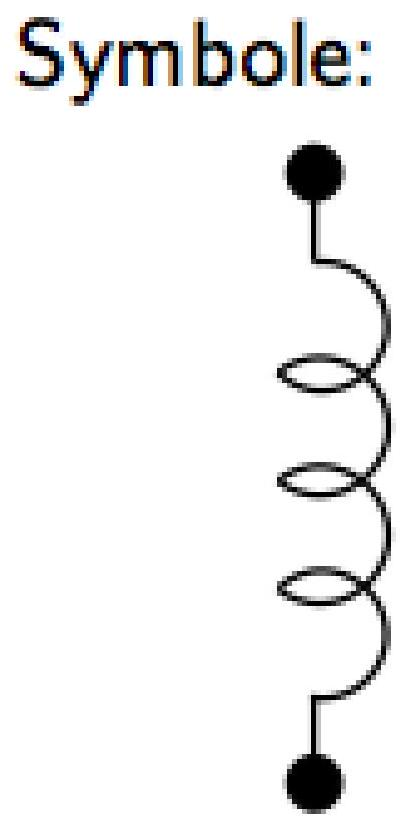
\includegraphics[width=\textwidth]{images/0aae1f8e-05fc-4834-a308-b46d85861175-29_822_415_1489_2711}\\
%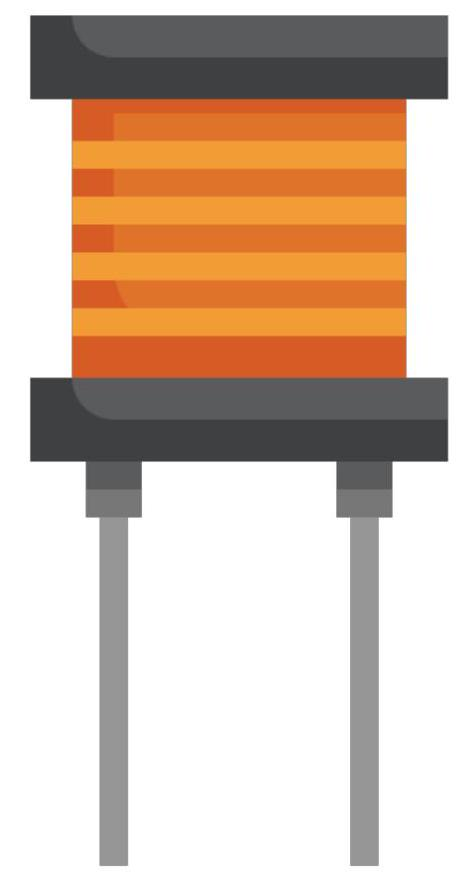
\includegraphics[width=\textwidth]{images/0aae1f8e-05fc-4834-a308-b46d85861175-29_886_466_159_3806}\\
%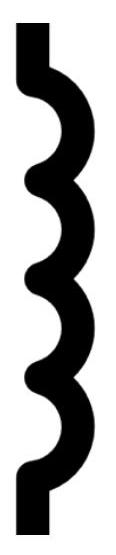
\includegraphics[width=\textwidth]{images/0aae1f8e-05fc-4834-a308-b46d85861175-29_555_116_1667_3736}
\end{frame}

\begin{frame}{Paramètres physiques d'une bobine et coefficient de self-induction}

Le coefficient de self-induction s'exprime, en fonction des paramètres physiques de la bobine par
$$
\boxed{L=\mu \frac{N^{2} S}{\ell}}
$$

où 
\begin{itemize}
  \item $\mu$ est la perméabilité magnétique du noyau
  \item $S$ est la surface d'une spire 
  \item $\ell$ est la longueur de la bobine.
\end{itemize}

Le coefficient de self-induction s'exprime en \alert{Henry}, dont le symbole est $H$.

\end{frame}

\begin{frame}{En régime non stationnaire}
Une variation du courant et donc du flux implique l'apparition d'une force contre-électromotrice aux bornes de la bobine (loi de Lenz).\\
Au niveau de la bobine :
\begin{itemize}
  \item le flux qui traverse les spires est variable
  \item selon la loi de Lenz, apparition d'une force contre-électromotrice $\frac{d \phi}{d t}$
  \item l'induction magnétique est variable à l'intérieur de la bobine
\end{itemize}

$$
\vec{\nabla} \times \vec{E}=-\frac{\partial \vec{B}}{\partial t}
$$

Ce flux et cette induction magnétique variables sont "confinés" à l'intérieur de l'élément : hypothèse des circuits localisés, pas de propagation.
\end{frame}

\begin{frame}{Modèle de la théorie des circuits}

On définit le \alert{flux} $\phi(t)$ associé à un dipôle par
$$
\phi(t)=\int_{-\infty}^{t} u(x) d x
$$

On appelle \alert{inductance} un dipôle tel que le flux $\phi$ induit par un courant $i$ le parcourant est une fonction de ce courant.
$$
\phi(t)=L i(t)
$$

\end{frame}

\begin{frame}{Relation entre $u$ et $i$ aux bornes d'une bobine}

  En pratique dans ce cours nous allons toujours considérer l'inductance $L$ linéaire et invariante, c'est-à-dire constante\footnote{En toute généralité : $L=f(u, i, t)$
}.

  \begin{columns}
  \begin{column}{0.45\textwidth}

  La tension $u(t)$ s'exprime par
  $$ u(t)=\frac{d \phi}{d t} $$

  Donc 
  $$ \boxed{u(t)=L \frac{d i(t)}{d t}} $$
  ou encore $i(t)=\frac{1}{L} \int_{-\infty}^{t} u(\tau) d \tau$.

  \end{column}
  \begin{column}{0.45\textwidth}
  Ces relations sont établies selon le sens conventionnel \\
  \begin{center}
    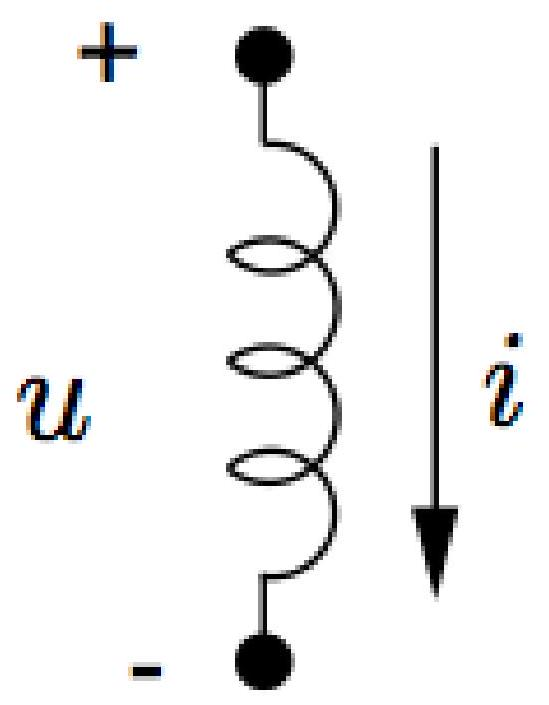
\includegraphics[width=0.3\textwidth]{images/0aae1f8e-05fc-4834-a308-b46d85861175-33_705_549_1320_2505}
  \end{center}
  \end{column}
\end{columns}

\end{frame}

\begin{frame}[allowframebreaks]{Elements physiques}
Solénoïde : \textbf{enroulement en cuivre} sur \textbf{matériau ferromagnétique}. 


\begin{columns}
  \begin{column}{0.5\textwidth}
    Modèle idéal de l'inductance plus éloigné de la réalité que pour $C$ et $R$ :
    \begin{itemize}
      \item pertes par effet Joule dans le conducteur\\
      \item effet pelliculaire aux hautes fréquences
      \item pertes dans le noyau ferromagnétique (hystérésis)
    \end{itemize}
  \end{column}
  \begin{column}{0.4\textwidth}
    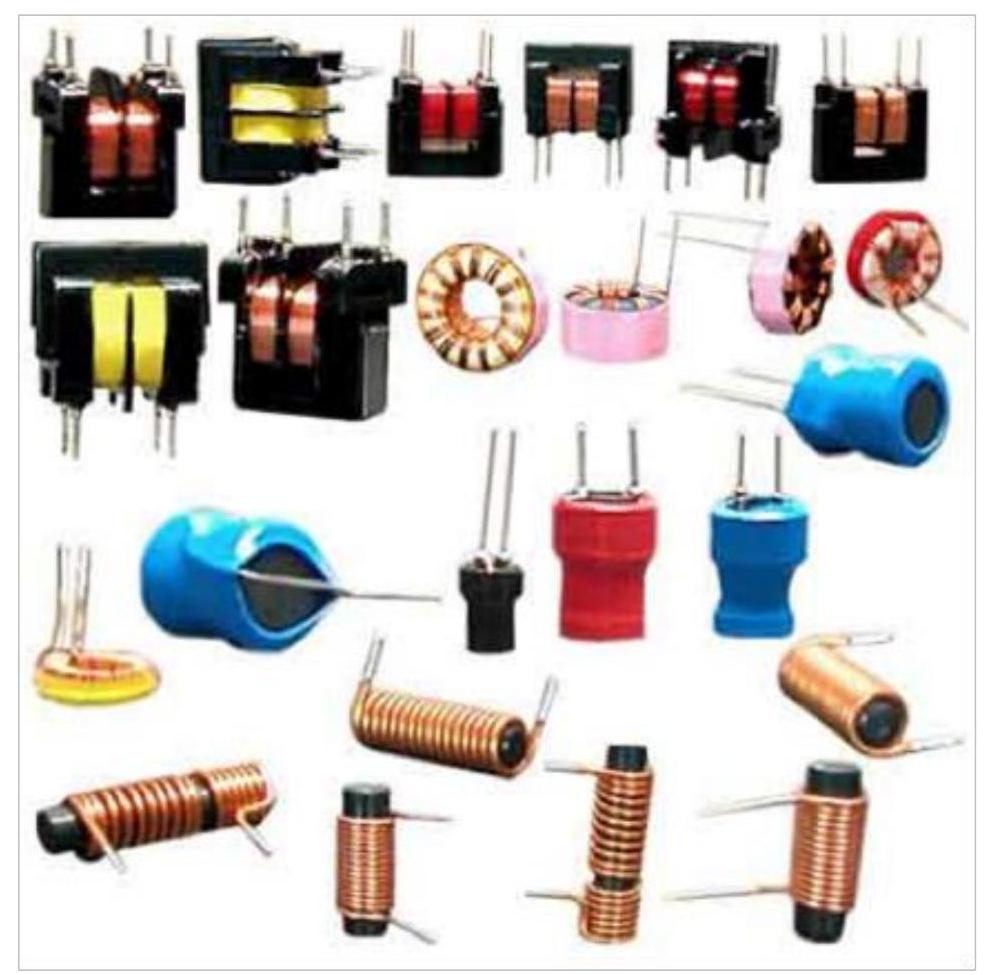
\includegraphics[width=0.9\textwidth]{images/0aae1f8e-05fc-4834-a308-b46d85861175-35_975_987_76_3431}
  \end{column}
\end{columns}

\begin{itemize}
  \item Des composants normalisés existent mais en moins grand nombre que pour $C$ et $R$ et de moins bonne précision.
  %\item Dans un circuit, éviter au maximum les bobines si possible (exemple filtres, filtres RC actifs plutôt que LC).
  \item Exemple d'inductance non autonome : capteur de position, une ferrite se déplace dans un bobinage, $L$ varie et caractérise la position.
  \item Linéarité : plusieurs causes de non-linéarite, hystérésis, saturation.
\end{itemize}

\end{frame}


\section{Propriétés des éléments R, L et C}

\begin{frame}[allowframebreaks]{Puissance absorbée par une résistance linéaire}
  
  \begin{columns}
  \begin{column}{0.45\textwidth}
    Convention moteur\\
    \begin{center}
      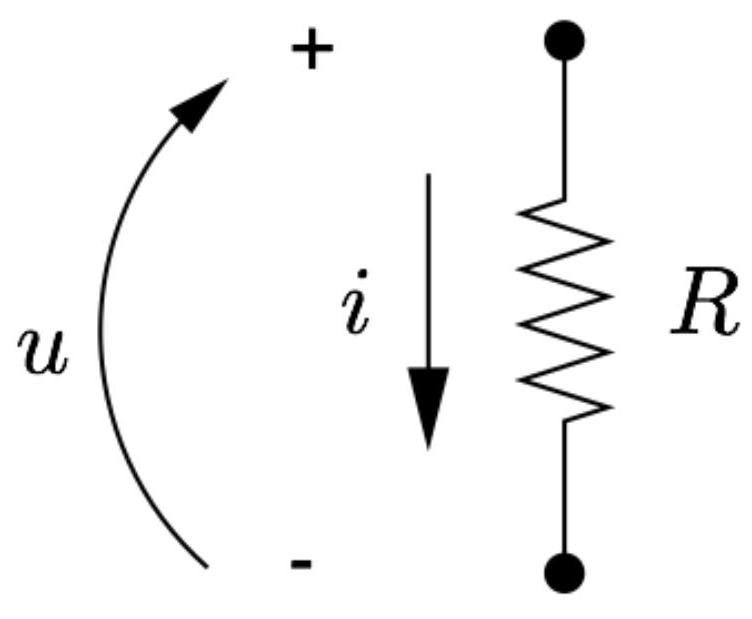
\includegraphics[width=0.3\textwidth]{images/0aae1f8e-05fc-4834-a308-b46d85861175-37_619_752_432_1171}
    \end{center}

    $$ u=R i$$
    
    $$
    \begin{aligned}
    p_{R}(t) & =u(t) i(t) \\
    & =R i(t) i(t)=R i^{2}(t) \geq 0
    \end{aligned}
    $$
  \end{column}
  \begin{column}{0.45\textwidth}
    Convention générateur\\

    \begin{center}
    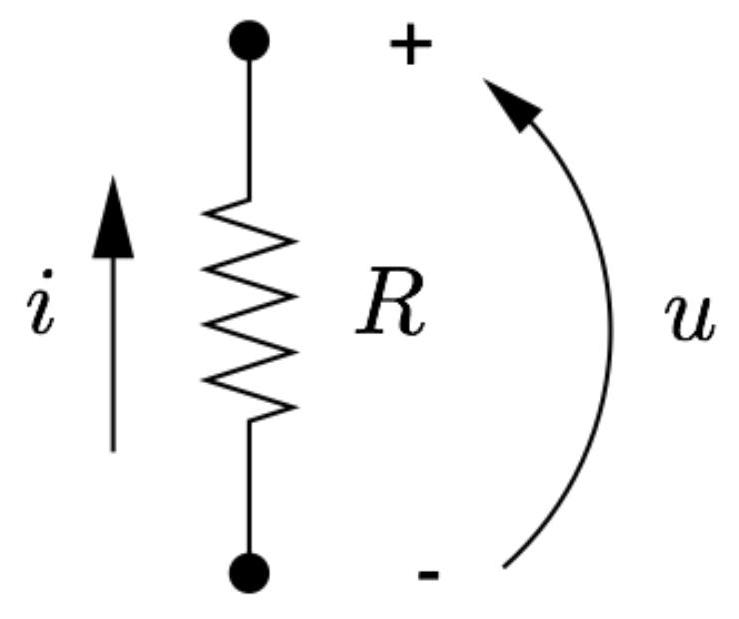
\includegraphics[width=0.3\textwidth]{images/0aae1f8e-05fc-4834-a308-b46d85861175-37_619_739_432_2457}
    \end{center}
    
    $$
    u= \mathcolor{red}{-}R i
    $$
    
    $$
    \begin{aligned}
    p_{R}(t) & = \mathcolor{red}{-}u(t) i(t) \\
    & =R i(t) i(t)=R i^{2}(t) \geq 0
    \end{aligned}
    $$
  \end{column}
\end{columns}

Energie dissipée :
$$
w_{R}(t)=\int_{-\infty}^{t} p(\tau) d \tau>0
$$

\begin{block}{Classification énergétiques d'un résistance}
  $R$ est un élément \textbf{passif} ( $w_{R}(t)>0$ ) et \textbf{dissipatif} ( $p_{R}(t) \geq 0$ ).
\end{block}
\end{frame}

\begin{frame}{Puissance absorbée par des éléments L et C linéaires}
  \begin{columns}
  \begin{column}{0.45\textwidth}
    \begin{center}
    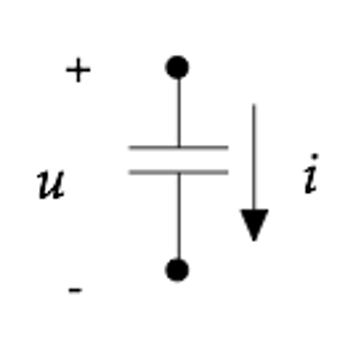
\includegraphics[width=0.2\textwidth]{images/C_conv_moteur.png}
    \end{center}
    $$
    \begin{aligned}
    i(t) & = C \frac{d u(t)}{d t} \\
    p_C(t) & =C u(t) \frac{d u(t)}{d t} \mathcolor{red}{\gtreqless 0} \\
    w_C(t) & =\int_{-\infty}^t C u(t) \frac{d u(t)}{d t} = \boxed{\frac{1}{2} C u^2(t) \geq 0}
    \end{aligned}
    $$
  \end{column}
  \begin{column}{0.45\textwidth}
    \begin{center}
    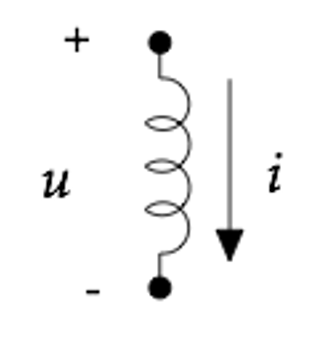
\includegraphics[width=0.2\textwidth]{images/L_conv_moteur.png}
    \end{center}
    $$
    \begin{aligned}
    u(t) & = L \frac{d i(t)}{d t} \\
    p_L(t) & =L i(t) \frac{d i(t)}{d t} \mathcolor{red}{\gtreqless 0} \\
    w_L(t) & =\int_{-\infty}^t L i(t) \frac{d i(t)}{d t}  = \boxed{\frac{1}{2} L i^2(t) \geq 0}
    \end{aligned}
    $$
  \end{column}
  \end{columns}
  \begin{block}{Classification énergétiques de $L$ et $C$}
  $L$ et $C$ sont donc des éléments \textbf{passifs} $(w(t) \geq 0)$, mais \textbf{non dissipatifs}, ils peuvent restituer de la puissance quand $(p(t)<0)$
  \end{block}

\end{frame}

\begin{frame}[allowframebreaks]{$C$ et $L$ ont une mémoire}
Soit un condensateur excité par un courant $i(t)$. On a

$$
u(t)=\frac{1}{C} \int_{-\infty}^{t} i(x) d x
$$

$u(t)$ dépend non seulement de $i$ à l'instant $t$ mais aussi de $i(x)$ pour $x<t$, soit de toute l"histoire" du système.

On a aussi :

$$
u(t)=u\left(t_{0}\right)+\frac{1}{C} \int_{t_{0}}^{t} i(x) d x
$$

$u\left(t_{0}\right)$ résume tout le passé du système de $\left[-\infty, t_{0}\right]$

De même pour une inductance excitée par une tension $u(t)$

$$
i(t)=\frac{1}{L} \int_{-\infty}^{t} u(x) d x \quad i(t)=i\left(t_{0}\right)+\frac{1}{L} \int_{t_{0}}^{t} u(x) d x
$$

\end{frame}

\begin{frame}[allowframebreaks]{Propriété de continuité}

  \begin{block}{Continuité de la tension aux bornes d'un condensateur}
    Si le courant $i(t)$ induit par un condensateur est borné $\forall t$, alors la tension aux bornes de ce condensateur est une grandeur continue.    
  \end{block}
Découle de la relation $ u=\frac{1}{C} \int_{-\infty}^{t} i(x) dx$

$u$ ne peut varier de manière instantanée aux bornes d'un condensateur. 
Sinon, courant infini (cas de l'impulsion de Dirac !):
\begin{itemize}
  \item mise sous tension brusque d'un condensateur
  \item court-circuiter un condensateur
\end{itemize}
Attention, on suppose ici les éléments idéaux, c-à-d sans pertes (voir point suivant). 


\textbf{En tenant compte des pertes}, le courant lors d'une mise sous tension brusque est très important mais reste borné !

\newpage
\begin{block}{Continuité du courant dans une bobine}
   Si la tension $u(t)$ aux bornes d'une inductance est bornée $\forall t$, alors le courant dans cette inductance est une grandeur continue.
\end{block}


Découle de la relation $i=\frac{1}{L} \int_{-\infty}^{t} u(x) dx$
\begin{itemize}
  \item $i$ ne peut varier de manière instantanée aux bornes d'une inductance
  \item Sinon : tension infinie (cas de l'impulsion de Dirac !)
  \item Difficulté de couper le courant dans un circuit inductif (arc!)
\end{itemize}
\end{frame}

\begin{frame}[allowframebreaks]{Exemple}
  Une inductance de 100 mH est alimentée par une source de courant délivrant un signal de courant de la forme :
  \begin{columns}
    \begin{column}{0.45\textwidth}
      $$
      i(t)= \begin{cases}0 & t<0 \\ 10 t e^{-5 t} & t>0\end{cases}
      $$
  \end{column}
  \begin{column}{0.25\textwidth}
    \begin{center}
    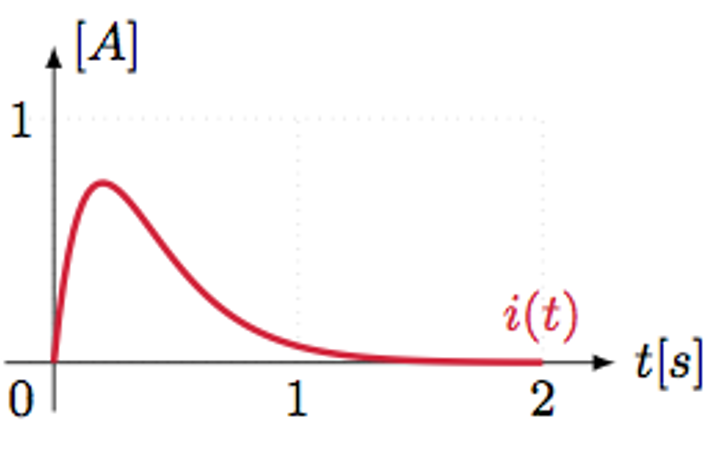
\includegraphics[width=\textwidth]{images/I_example.png}
    \end{center}
  \end{column}
\end{columns}

\begin{block}{Question}
  Que vaut $u(t)$ ? 
\end{block}

\newpage
  \begin{columns}
    \begin{column}{0.45\textwidth}
      Donc
      $$
      u(t)= \begin{cases}0 & t<0 \\ e^{-5 t}(1-5 t) & t>0\end{cases}
      $$
  \end{column}
  \begin{column}{0.25\textwidth}
    \begin{center}
    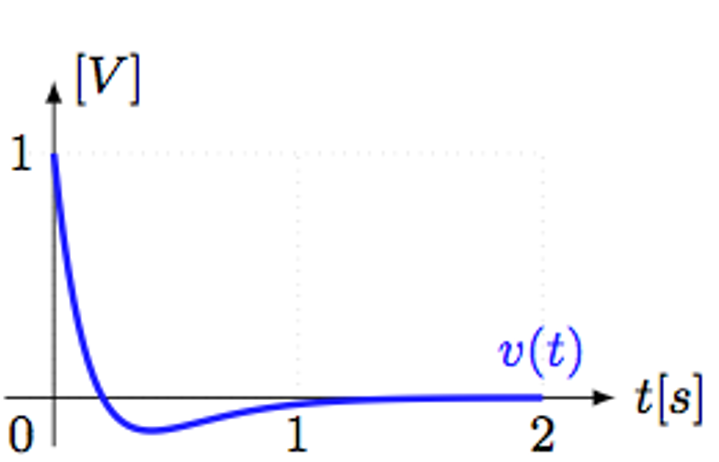
\includegraphics[width=\textwidth]{images/V_example.png}
    \end{center}
  \end{column}
\end{columns}


\begin{block}{Question}
  Que valent la puissance $p(t)$  et l'énergie $w(t)$ ? 
\end{block}
\newpage

  \begin{columns}
    \begin{column}{0.45\textwidth}
      $$
      p(t)= \begin{cases}0 & t<0 \\ 10 t(1-5 t) e^{-10 t} & t>0\end{cases}
      $$

      $$
      w(t)= \begin{cases}0 & t<0 \\ 5 t^{2} e^{-10 t} & t>0\end{cases}
      $$
  \end{column}
  \begin{column}{0.25\textwidth}
    \begin{center}
    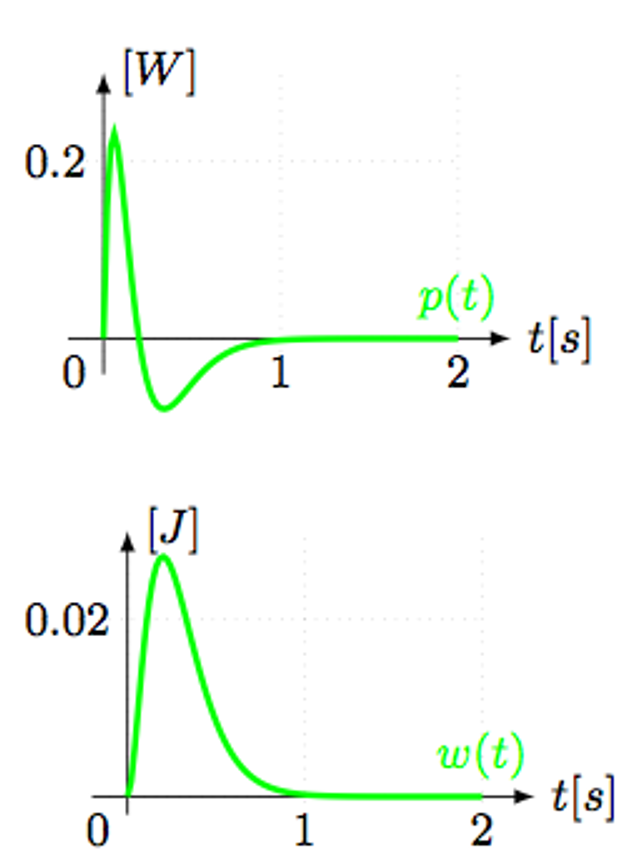
\includegraphics[width=\textwidth]{images/P_et_L.png}
    \end{center}
  \end{column}
\end{columns}
\newpage
\begin{itemize}
  \item Dans l'intervalle [ $0-0.2$ ] s , l'inductance stocke une certaine énergie
  \item dans l'intervalle $[0.2-\infty] \mathrm{s}$, cette énergie est restituée
\end{itemize}

On a :
\begin{itemize}
  \item $w(t) \geq 0 \quad \forall t$ : élément passif
  \item $w(\infty) \rightarrow 0$ : finalement aucune énergie n'est dissipée
\end{itemize}
\end{frame}